\section{Online deployment and performance}%
\label{sec:operation}


 The \rnn{} algorithm was implemented in three stages during 2017--2018 in LHC \RunTwo:

\begin{enumerate}[i]
  %\item A development stage up to early 2017, where the \rnn{}'s performance was estimated by rerunning the trigger decision offline.
  
  \item The commissioning stage in early 2017 runs ($5.4~\ifb$), where all primary triggers were duplicated and both the \rnn{} and cut-based algorithm run in parallel in the \fastcalo{} stage of the HLT.
  
\item The operation stage, starting after Technical Stop~1 (TS1) in 2017. 
Triggers using \rnn{} were used as the main triggers, and a small set of cut-based triggers was kept active solely for validation. 
Final validation of the \rnn{} was performed by comparing the main triggers and the cut-based triggers from this period ($39.0~\ifb$) as shown in Section~\ref{ssec:deploy_ringer} and Section~\ref{sec:off_ana}.

\item The \rnn{}-only stage, during 2018. Duplicated cut-based triggers were removed. The performance of the Neural-Ringer in 2018 is presented in Section~\ref{ssec:deploy_ringer}. The results presented for this case are consistent with the second part of Run 2 and the full Run 3 scenario.
    
\end{enumerate}

This section reports \rnn{}'s operational performance in each of these periods. In addition, the observed impact on CPU usage is discussed in Section~\ref{ssec:cpu_reduction}.

\subsection{Measurement of the electron trigger efficiency}

The electron trigger efficiency is measured using the tag-and-probe method, which provides a sample of electrons selected without bias from the trigger decision. This technique allows unbiased estimation of the trigger performance by identifying probe electrons in events where a tag electron satisfies stringent offline and trigger requirements.

The efficiency is defined as the fraction of probe electrons that are accepted by the trigger, among those that pass the full offline selection:

\begin{equation}
    \epsilon_{\text{trigger}} = \frac{N_{\text{trigger} \cap \text{offline}}}{N_{\text{offline}}}
\end{equation}

where \( N_{\text{trigger} \cap \text{offline}} \) is the number of probe electrons that pass both the offline selection and are accepted by the trigger, and \( N_{\text{offline}} \) is the total number of probe electrons passing the offline selection.


%where $\epsilon_{EMclus}$ is the probability to reconstruct a cluster into the EM2 given a truth electron produced at generator level from MC simulation. 
%This efficiency is computed as the ratio of the number of EM-clusters that matches with an electron, $N_{clusters}$, and the number of produced electrons, $N_{all}$. 
%The reconstructed efficiency, $\epsilon_{reco}$, is the performance of the track reconstruction and its association with the cluster. 
%It is obtained from the number of reconstructed electron candidates with track association, $N_{reco}$, divided by the number of EM clusters candidates, $N_{clusters}$. 

%The identification efficiency, $\epsilon_{id}$, is the probability of a reconstructed electron to satisfy a certain offline identification criteria. It is defined as the number of identified and reconstructed electron candidates, $N_{id}$, divided by $N_{reco}$. The isolation efficiency, $\epsilon_{iso}$, is the probability of an offline identified electron to pass requirements on the track or calorimeter isolation. It is calculated as the number of offline identified electron candidates satisfying the isolation, identification, and reconstruction requirements, $N_{iso}$, divided by $N_{id}$.

%Finally, the trigger efficiency, $\epsilon_{trigger}$, is calculated as the number of reconstructed, identified and isolated electron candidates passing the trigger requirements, $N_{trig}$, divided by $N_{iso}$. 
%Only $\epsilon_{trigger}$ efficiency is further discussed in this paper.

%All efficiencies except $\epsilon_{EMclus}$ are estimated directly from data using tag-and-probe methods to select from unbiased samples of probe electrons produced in the decays of well-known resonances, such as $Z\rightarrow e^{+}e^{-}$, unbiased samples of electrons produced in the particle's decay. 
%All efficiencies, except for $\epsilon_{EMclus}$, are estimated directly from data using the tag-and-probe method. 
%This approach selects unbiased samples of probe electrons from decays of well-known resonances, such as $Z \rightarrow e^{+}e^{-}$, or from unbiased electron samples produced in the particle's decay.


%For all trigger efficiencies discussed further, the operating point of the offline identification criteria used to select reconstructed probe electron candidates generally follows the equivalent operating point defined in the trigger requirement (e.g, a trigger with 'tight' online LH identification as requirement uses a 'tight' offline LH identification to select reconstructed probe electrons estimated from data using tag-and-probe $Z\rightarrow e^+e^-$ method.).


\subsection{Assessment and deployment of Neural Ringer trigger Algorithm during Run 2 operation}\label{ssec:deploy_ringer}


The operation of \rnn{} commenced after the technical stop period (TS1) occurred in mid-2017. For monitoring purposes, a single-electron trigger was used. This trigger requires $E_T > 28$ GeV, with the selection criteria \enquote{tight} and with \enquote{loose} isolation criteria.

Signal efficiencies for both cut-based and \rnn{} triggers, evaluated for \tnp{} electron candidates from 2017 data, are compared in Figure~\ref{fig:2017_e28_after_ts1}, where one can see both trigger efficiencies with respect to the offline Tight identification working point as a function of \et{}, \eta{} and \avgmu{}. The results show no significant differences, on the order of a few per mille, between the two algorithms. Although a slight efficiency loss is observed at higher \avgmu{} values in Figure~\ref{fig:e28_comp_mu} for the \rnn{} trigger, the overall electron efficiency was maintained nearly constant, consistent with the target efficiency of the \rnn{} algorithm’s training. The observed efficiency loss occurs after the application of the linear threshold correction at $\avgmu=40$ in 2017.

%Although a slight efficiency loss is observed at higher  \avgmu{} values in Figure~\ref{fig:e28_comp_mu} for the \rnn{} trigger, the overall electron efficiency was maintained nearly constant, consistent with the objective of the \rnn{} algorithm’s training. This strategy is further validated by the results. The observed efficiency loss occurs after the application of the linear threshold correction at $\avgmu=40$ in 2017.



Other important results were assessed by comparing the trigger efficiencies in the 2017 collision data collected before and after switching to the \rnn{} algorithms. As shown in Figure~\ref{fig:2017_electron_triggers}, the \rnn{} signal detection efficiency was approximately the same as the cut-based selection for the three trigger setups evaluated. One of these triggers requires an electron candidate with $\ET > 17$~GeV, seeded by the first-level trigger with $\ET > 15$ GeV, and satisfying the loosest identification criteria (lhvloose). 
On the other hand, another requires an electron candidate with $\ET>26$~GeV satisfying \enquote{tight} identification (lhtight) with \enquote{loose} isolation (ivarloose), and the last requires an electron candidate with $\ET>60$~GeV satisfying \enquote{medium} identification (lhmedium). 
The electron efficiency was kept nearly unchanged for these relevant single-electron triggers. 
%As mentioned above, the results in Figure~\ref{fig:2017_electron_triggers} are computed for two different data-taking periods: one with, and the other without, the \rnn{} algorithm. 



\begin{figure}[h!tb]
  
  \begin{subfigure}[c]{.49\textwidth}
  \centering
  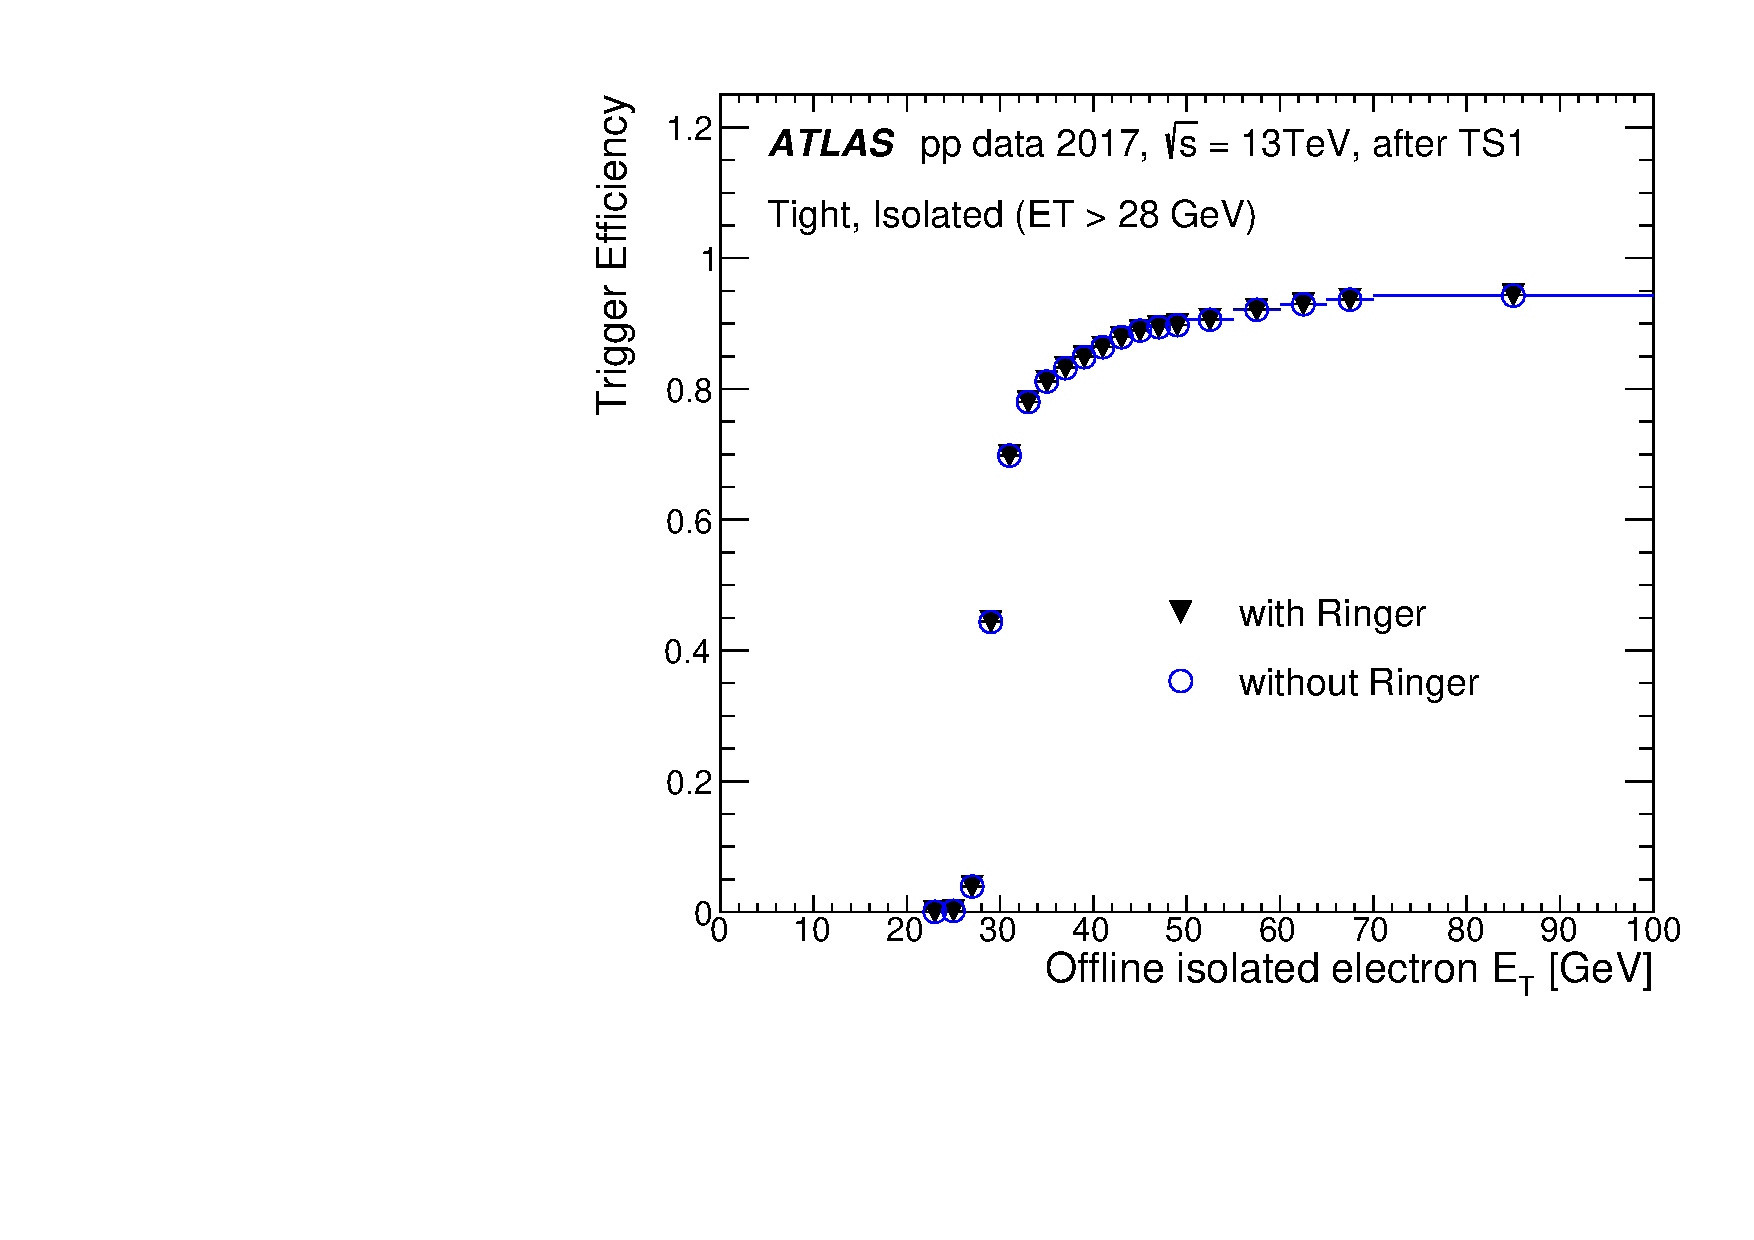
\includegraphics[width=\textwidth]{figures/efficiencies/eff_EGAM1_e28_ringer_and_noringer_2017_after_ts1_HLT_et.pdf}
  \caption{}
  \end{subfigure}
  %
  \begin{subfigure}[c]{.49\textwidth}
  \centering
  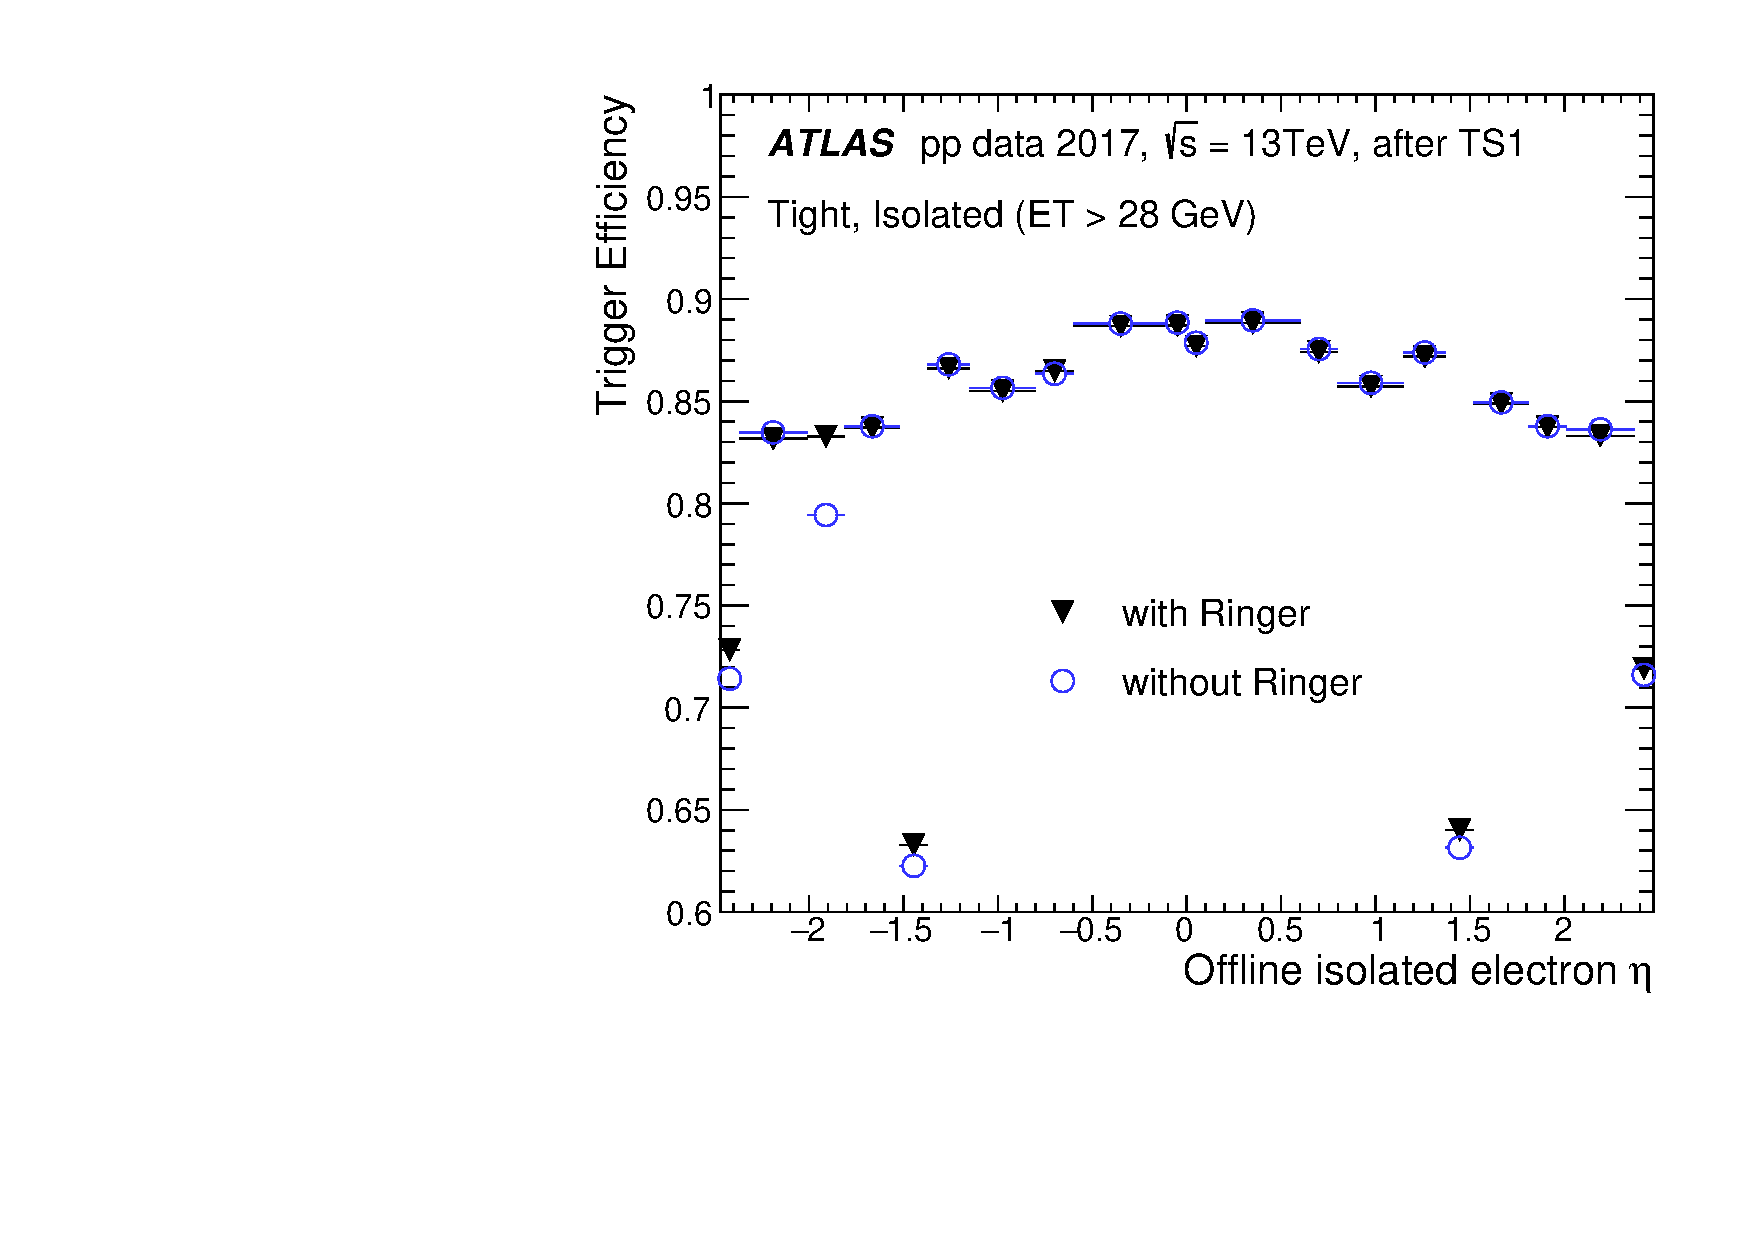
\includegraphics[width=\textwidth]{figures/efficiencies/eff_EGAM1_e28_ringer_and_noringer_2017_after_ts1_HLT_eta.pdf}
  \caption{}
  \end{subfigure}\\
  %
  \centering
  \begin{subfigure}[c]{.49\textwidth}
  \centering
  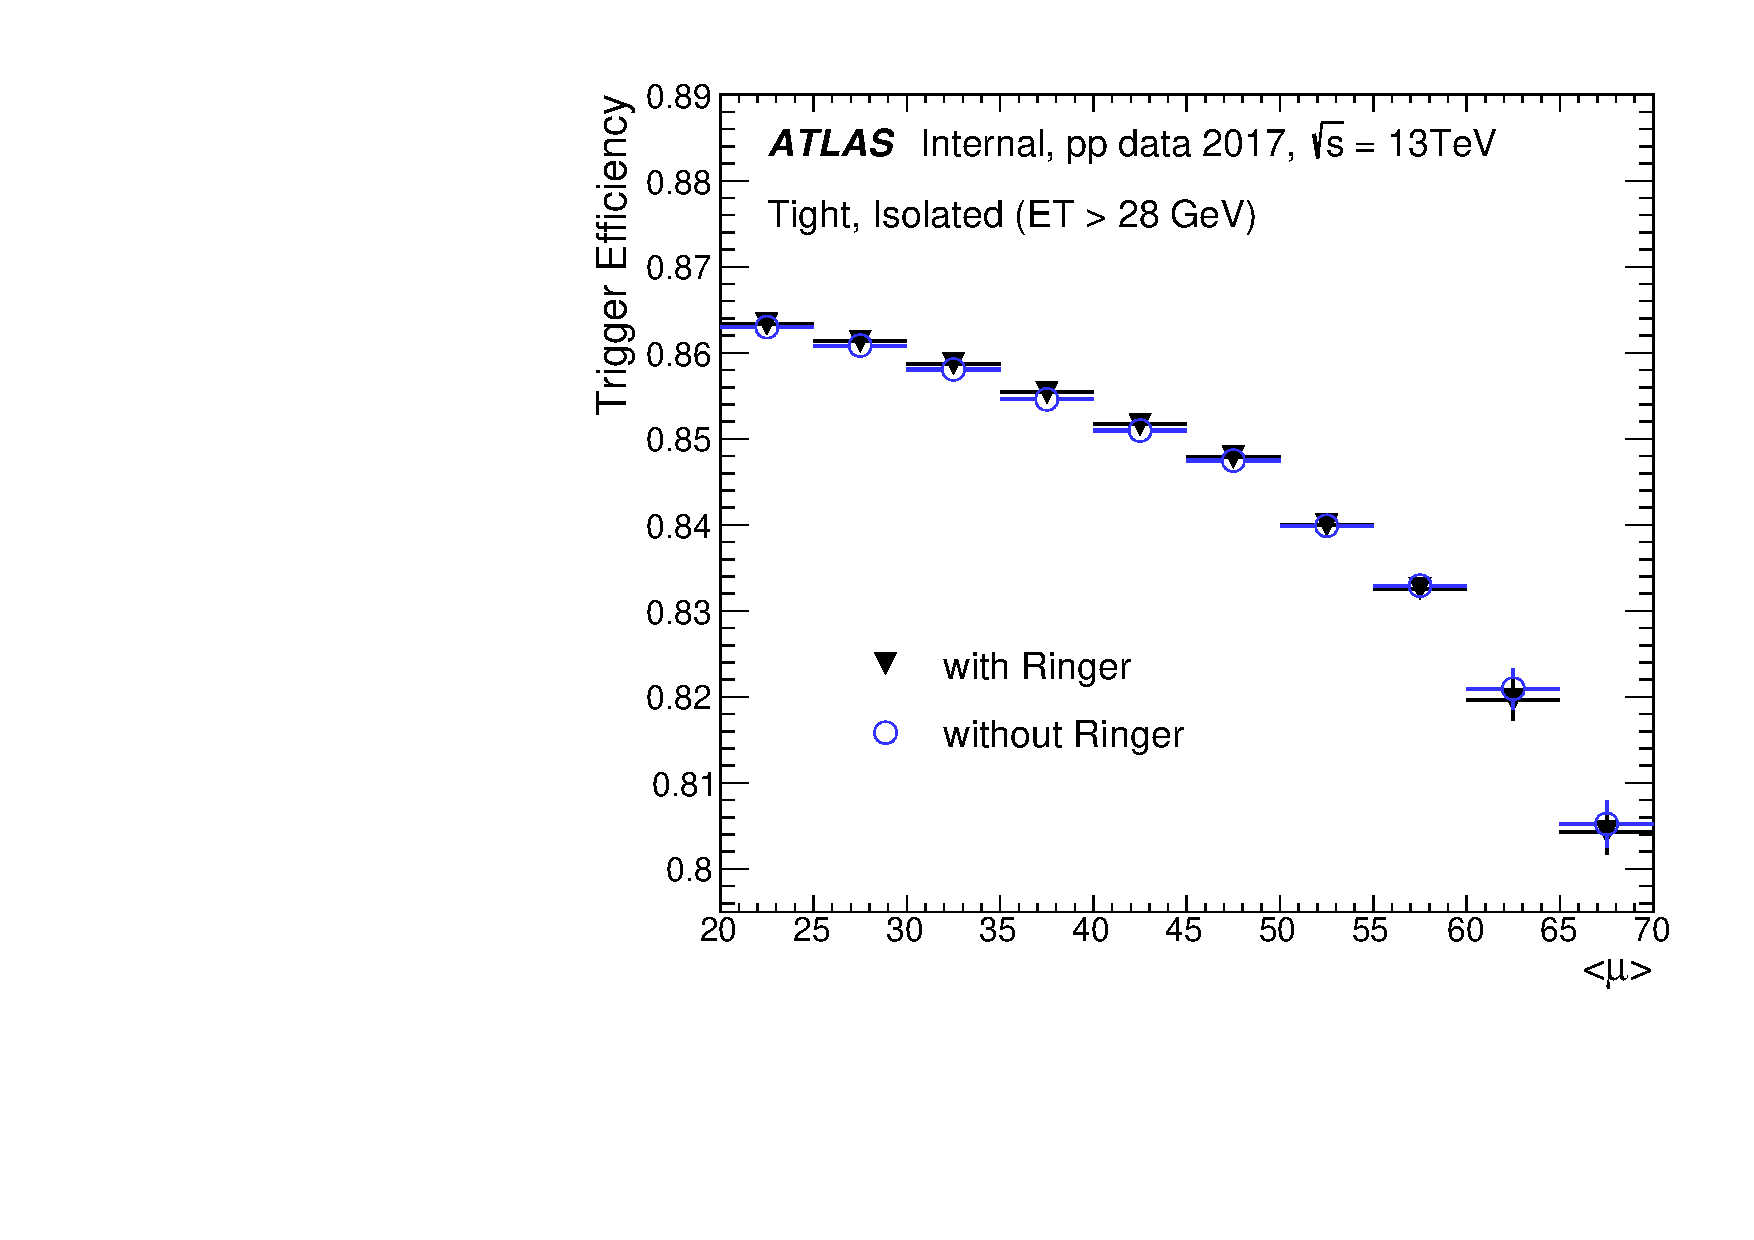
\includegraphics[width=\textwidth]{figures/efficiencies/eff_EGAM1_e28_ringer_and_noringer_2017_after_ts1_HLT_mu.pdf}
  \caption{}%
  \label{fig:e28_comp_mu}
  \end{subfigure}
  
  \caption{
     The efficiency of $\et{} > \SI{28}{\GeV}$ single-isolated-electron triggers with the \rnn{} algorithm and with the cut-based algorithms as a function of the offline electron (a) \et{}, (b) \eta{}, and (c) \avgmu{} after its deployment in July 2017. Efficiency is given with respect to the offline Tight identification working point. For (b) and (c), only offline candidates with $\et{} > \SI{29}{\GeV}$ are used.
  }
  \label{fig:2017_e28_after_ts1}
\end{figure}




\begin{figure}[h!tb]
  
 \begin{subfigure}[c]{.49\textwidth}
  \centering
  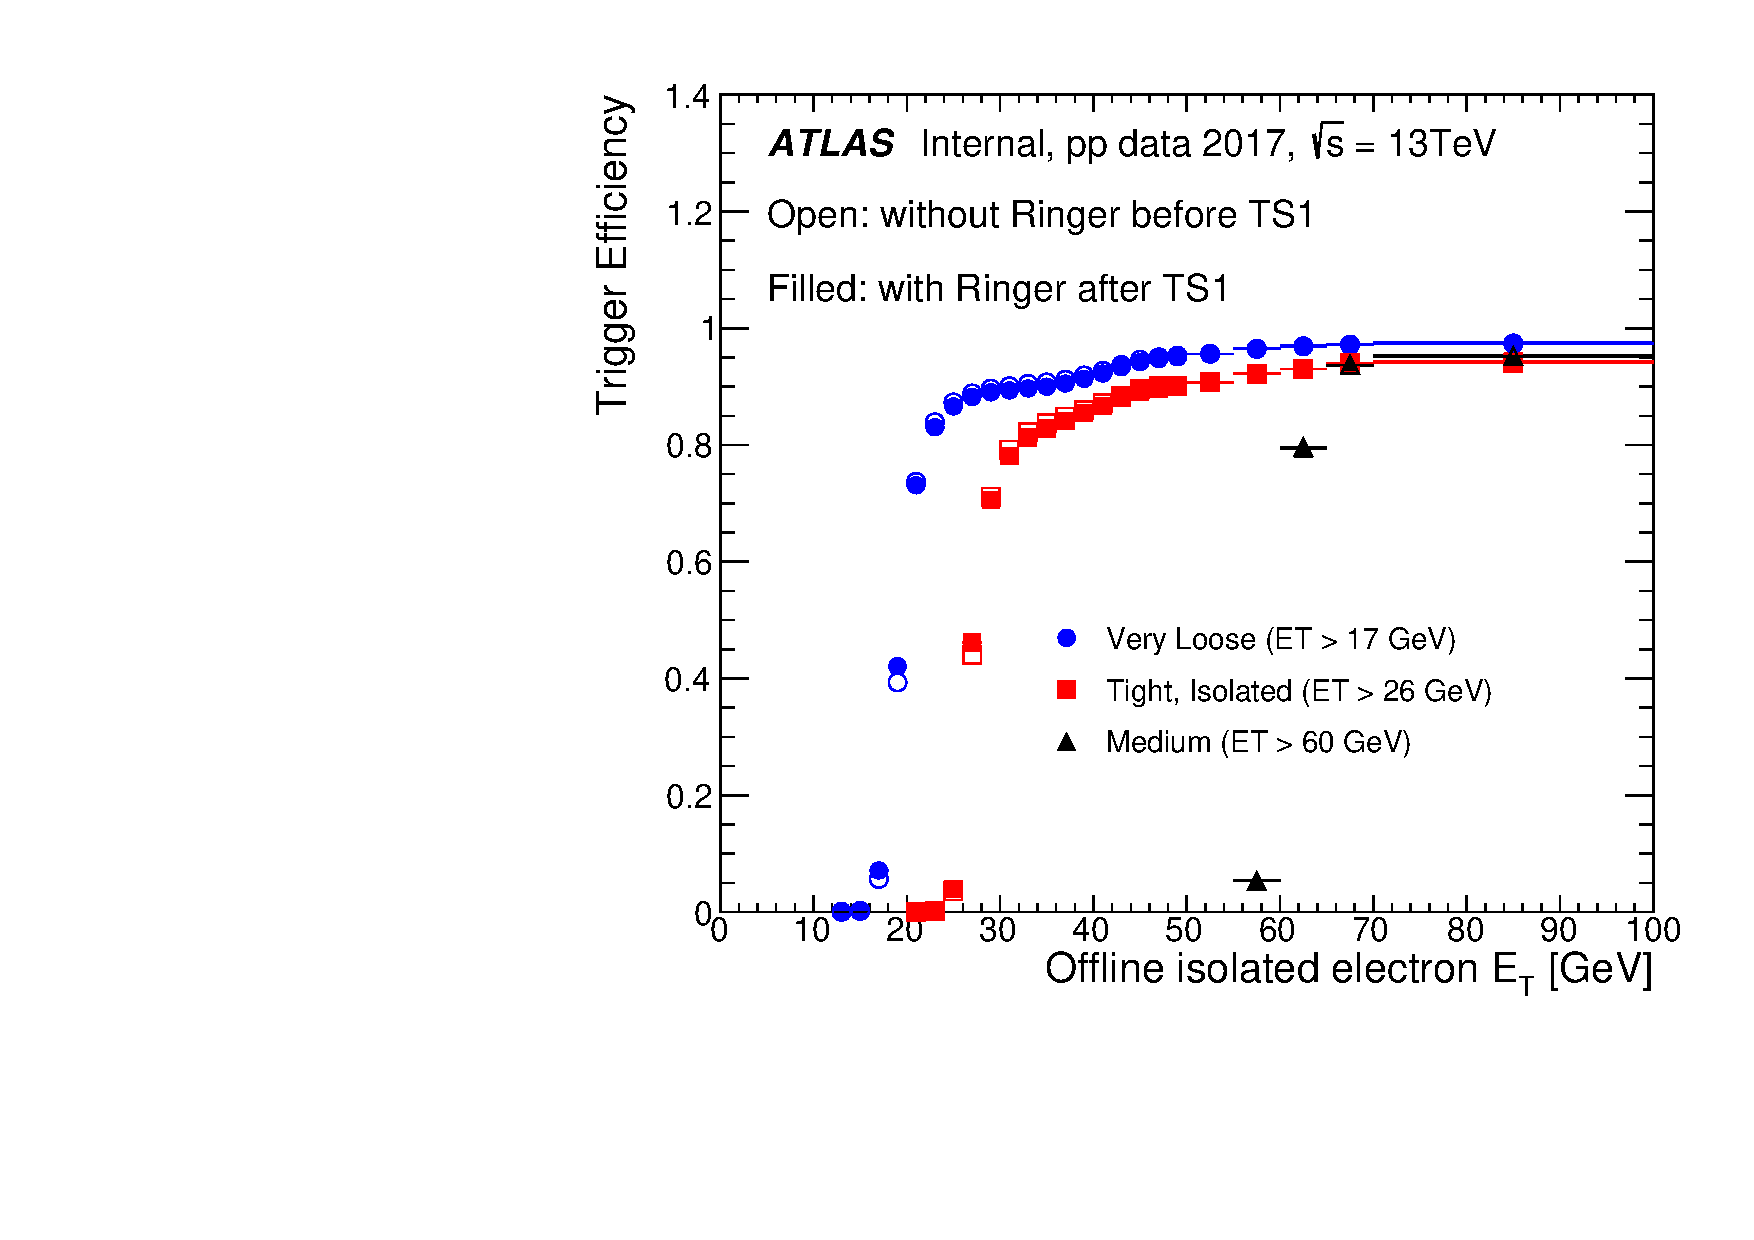
\includegraphics[width=\textwidth]{figures/efficiencies/eff_EGAM1_e17_e26_e60_2017_before_and_after_ts1_et.pdf}
  \caption{}%
  \end{subfigure}
  %
  \begin{subfigure}[c]{.49\textwidth}
  \centering
  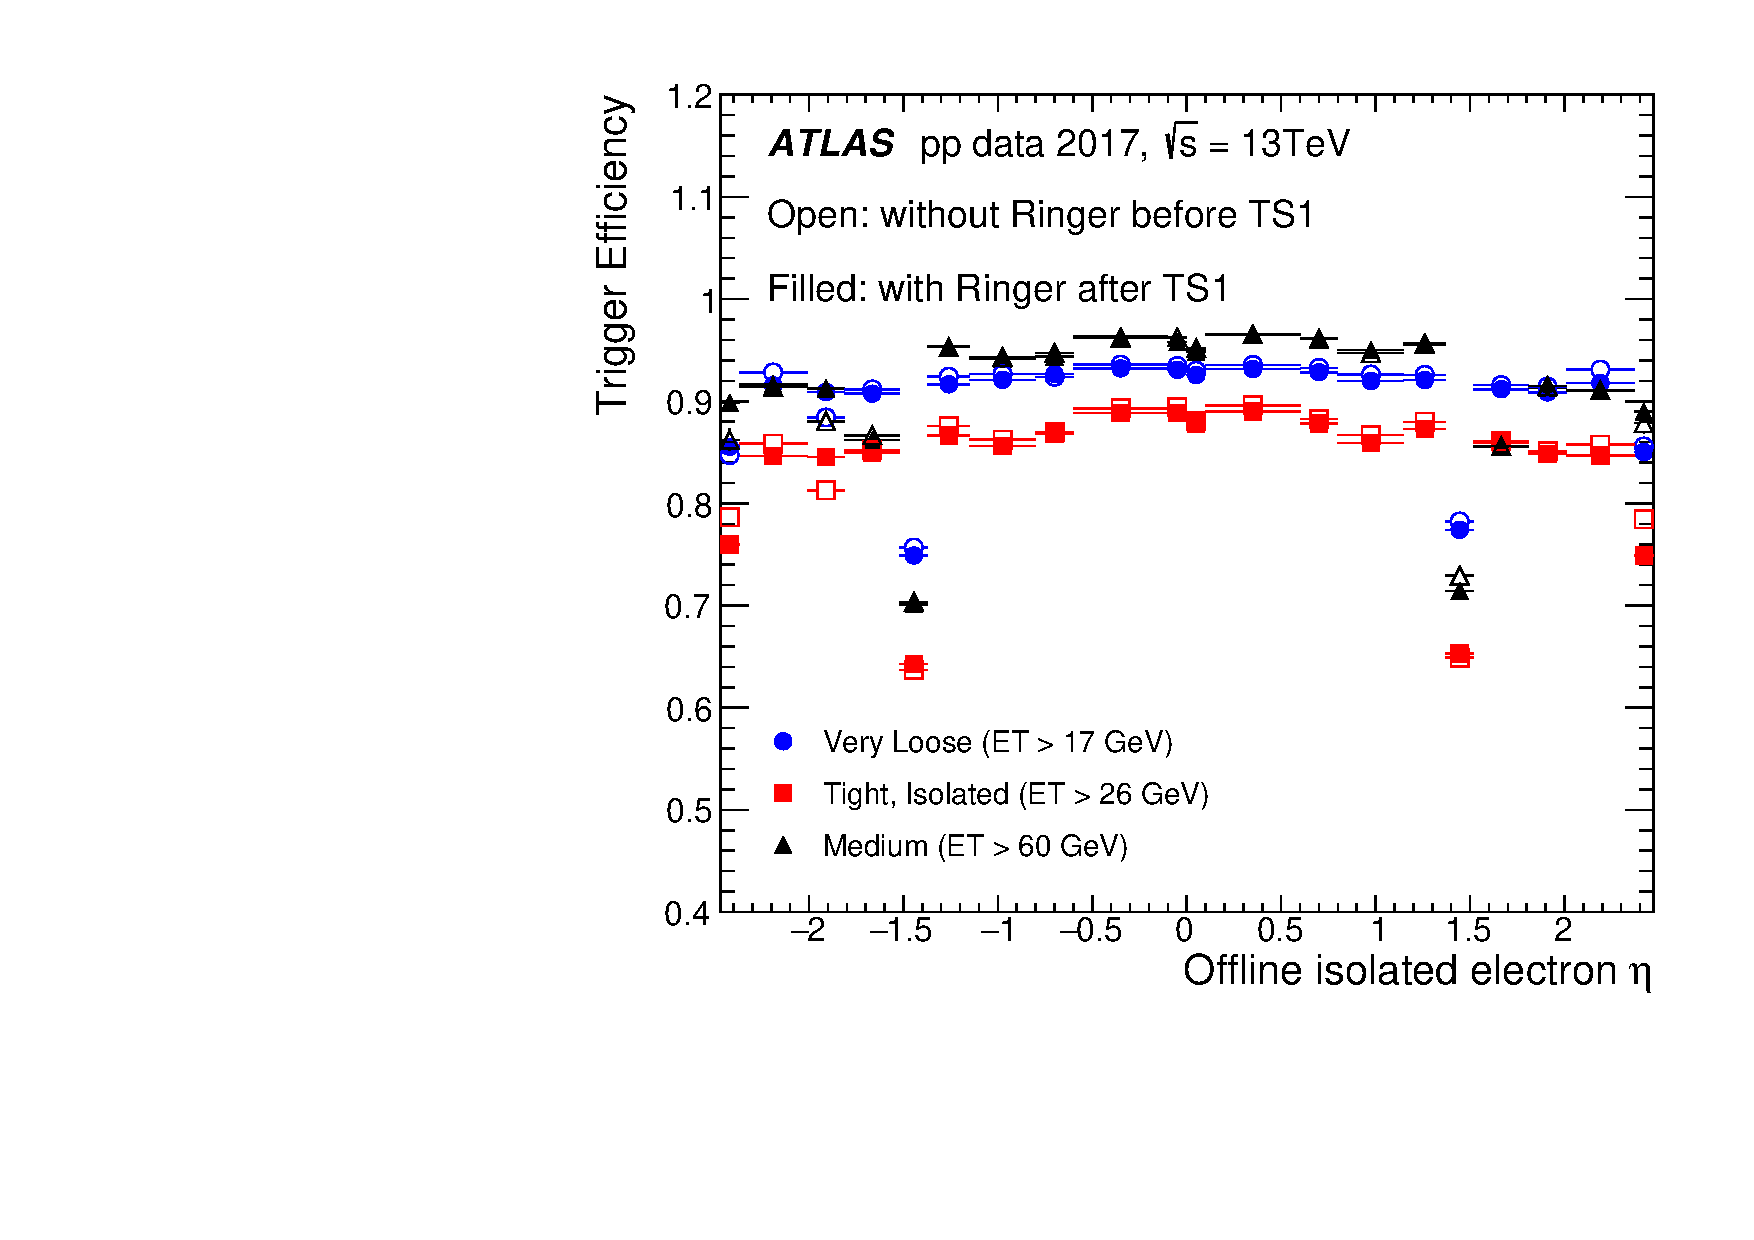
\includegraphics[width=\textwidth]{figures/efficiencies/eff_EGAM1_e17_e26_e60_2017_before_and_after_ts1_eta.pdf}
  \caption{}%
  \end{subfigure}
  
  \caption{
  Efficiency of three single-electron triggers as a function of (a) \et and (b) \eta for 2017 collision data. Open (filled) markers show the efficiency measurements in runs before (after) the deployment of the \rnn{}, thus referring to triggers executed without (with) the \rnn{} algorithm.}
  \label{fig:2017_electron_triggers}
\end{figure}


The presence of duplicated triggers, one configured with the \rnn{} algorithm and the other cut-based, allowed a direct comparison of their rates for fake electron candidates in collision data. 
%The power of the \rnn{} algorithm is made clear by examining the behaviour of the duplicated trigger for fake electron candidates in collision data. 
With the \rnn, the overall fake-electron rate is reduced by a factor of 13.75 at the \fastcalo step. It can be seen on the left side of Figure~\ref{fig:2017_fake_triggers_after_ts1} that the improvement at the \fastcalo step is similar for all regions in the evaluation with respect to $\ET$, $\eta$, and $\langle \mu \rangle$ variables, which is particularly interesting when considering the low \et{} and endcap regions. Besides improving early fake-electron rejection, the use of the \rnn{} also resulted in a factor of two reduction in the final fake-electron rate from the HLT (see right side of Figure~\ref{fig:2017_fake_triggers_after_ts1}), mostly coming from the calorimeter's barrel-endcap transition regions.


\begin{figure}[h!tb]
  \begin{subfigure}[c]{0.49\textwidth}
  \centering
  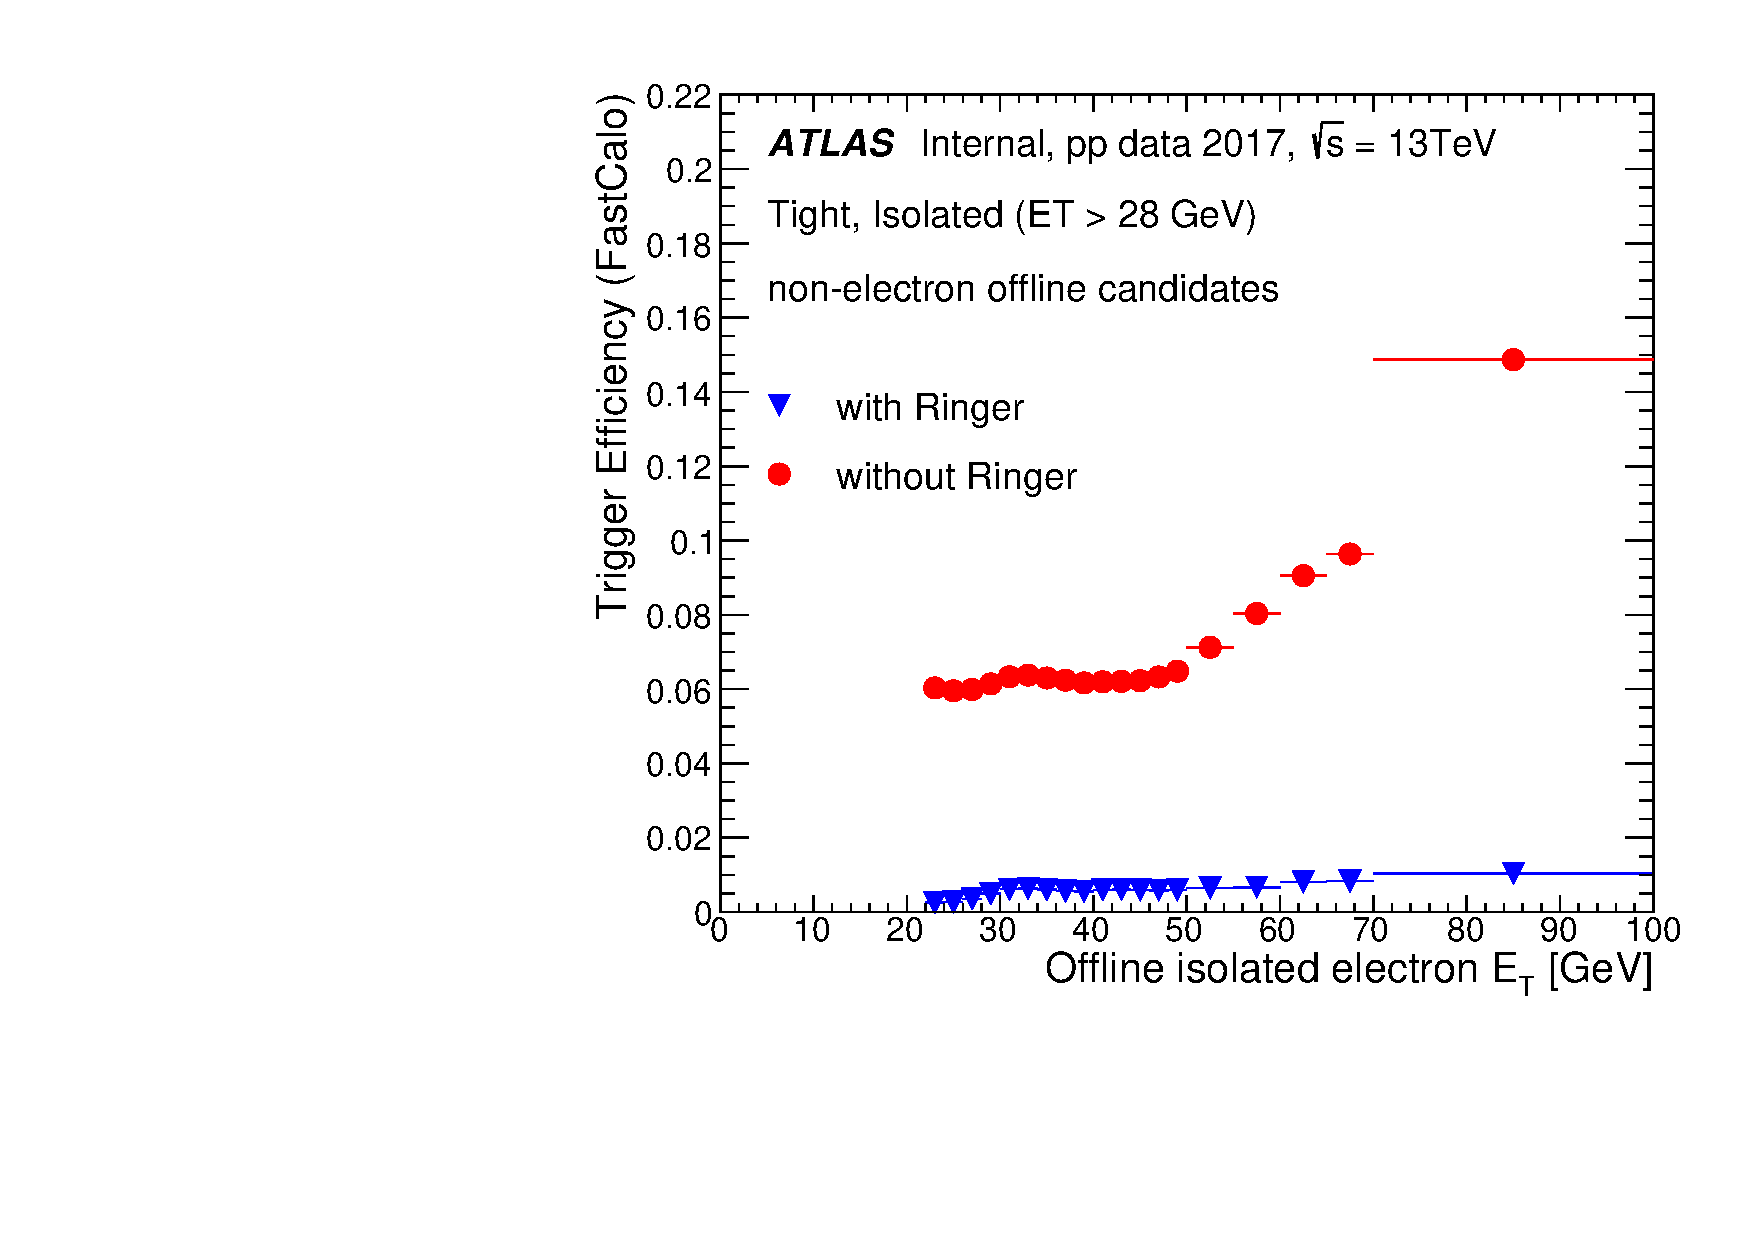
\includegraphics[width=\textwidth]{figures/efficiencies/eff_EGAM7_e28_ringer_and_noringer_2017_after_ts1_L2Calo_et.pdf}
  \caption{}
  \end{subfigure}
  %
  \begin{subfigure}[c]{.49\textwidth}
  \centering
  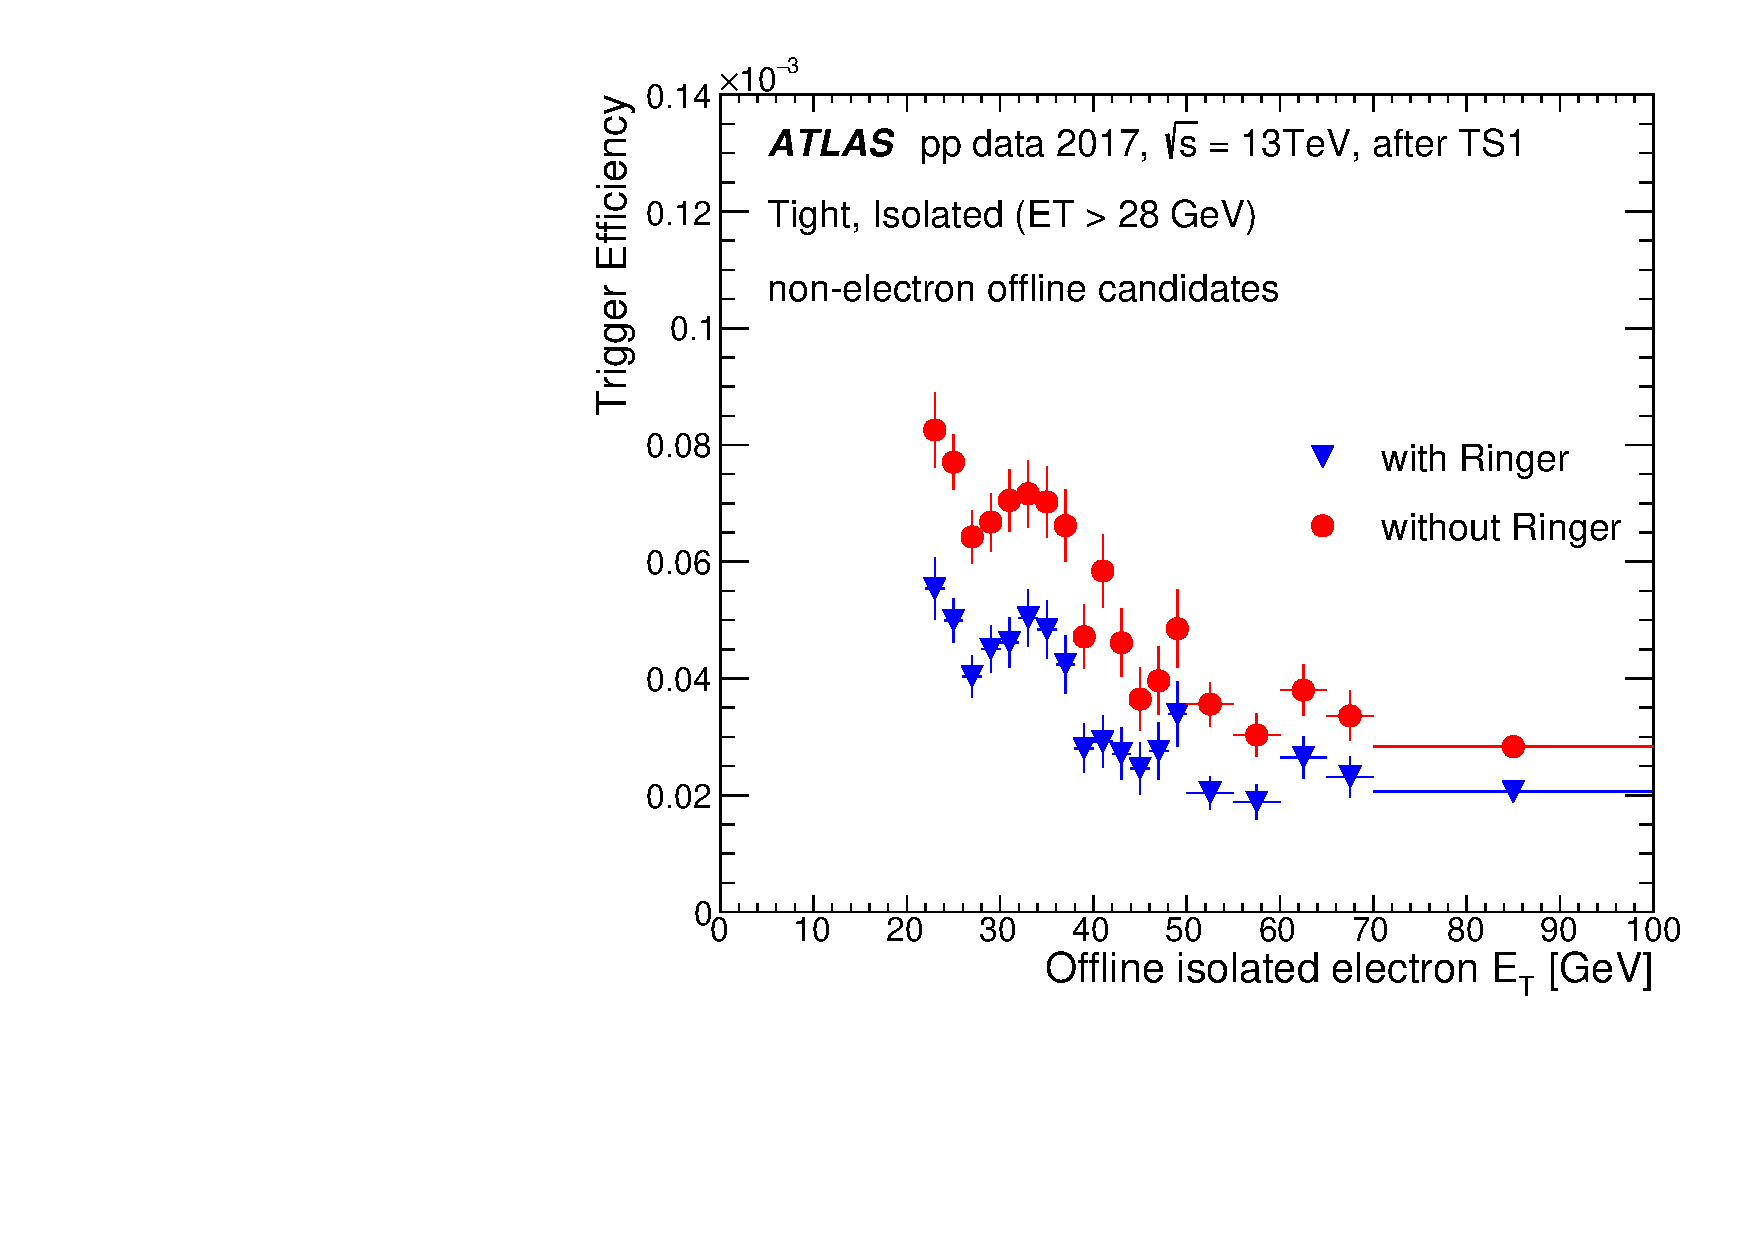
\includegraphics[width=\textwidth]{figures/efficiencies/eff_EGAM7_e28_ringer_and_noringer_2017_after_ts1_HLT_et.pdf}
  \caption{}
  \end{subfigure}\\
  %
  \begin{subfigure}[c]{.49\textwidth}
  \centering
  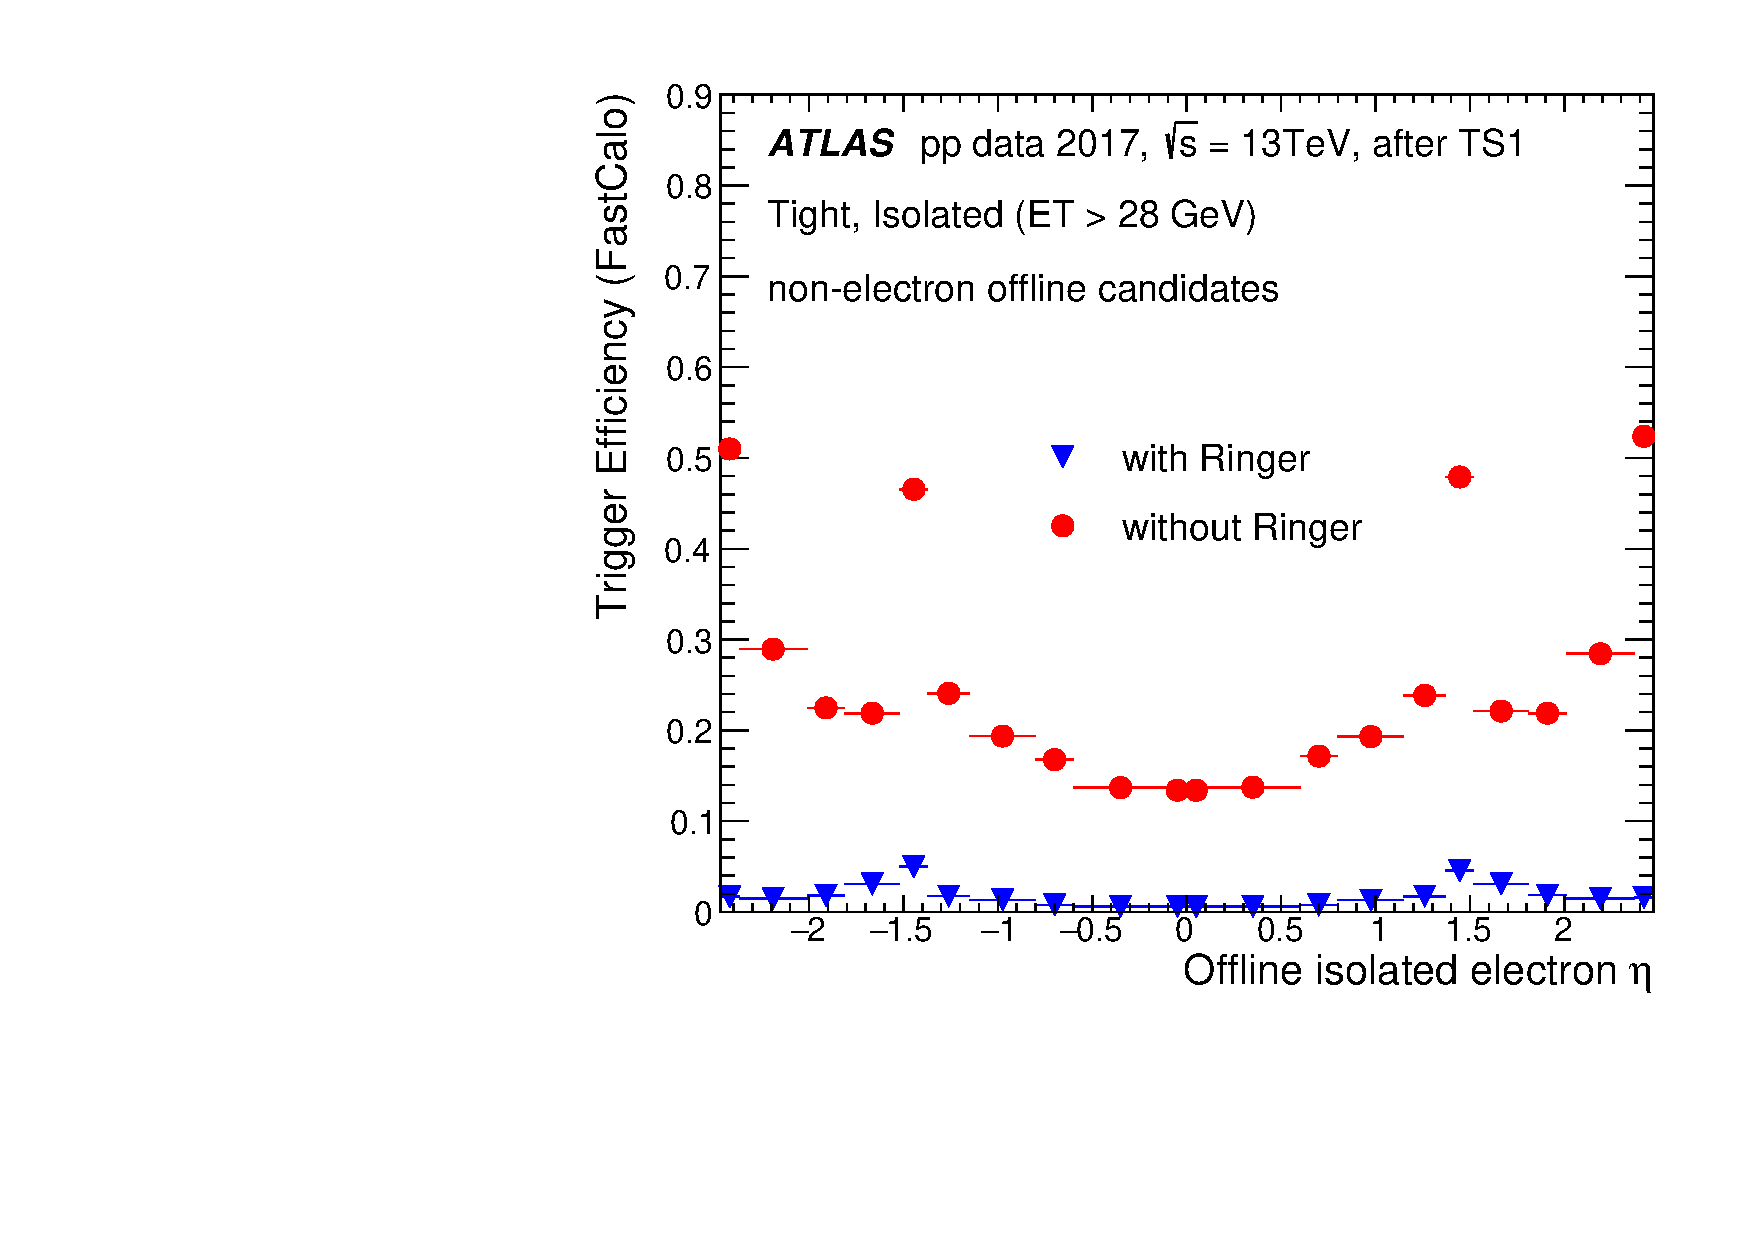
\includegraphics[width=\textwidth]{figures/efficiencies/eff_EGAM7_e28_ringer_and_noringer_2017_after_ts1_L2Calo_eta.pdf}
  \caption{}
  \end{subfigure}
  %
  \begin{subfigure}[c]{.49\textwidth}
  \centering
  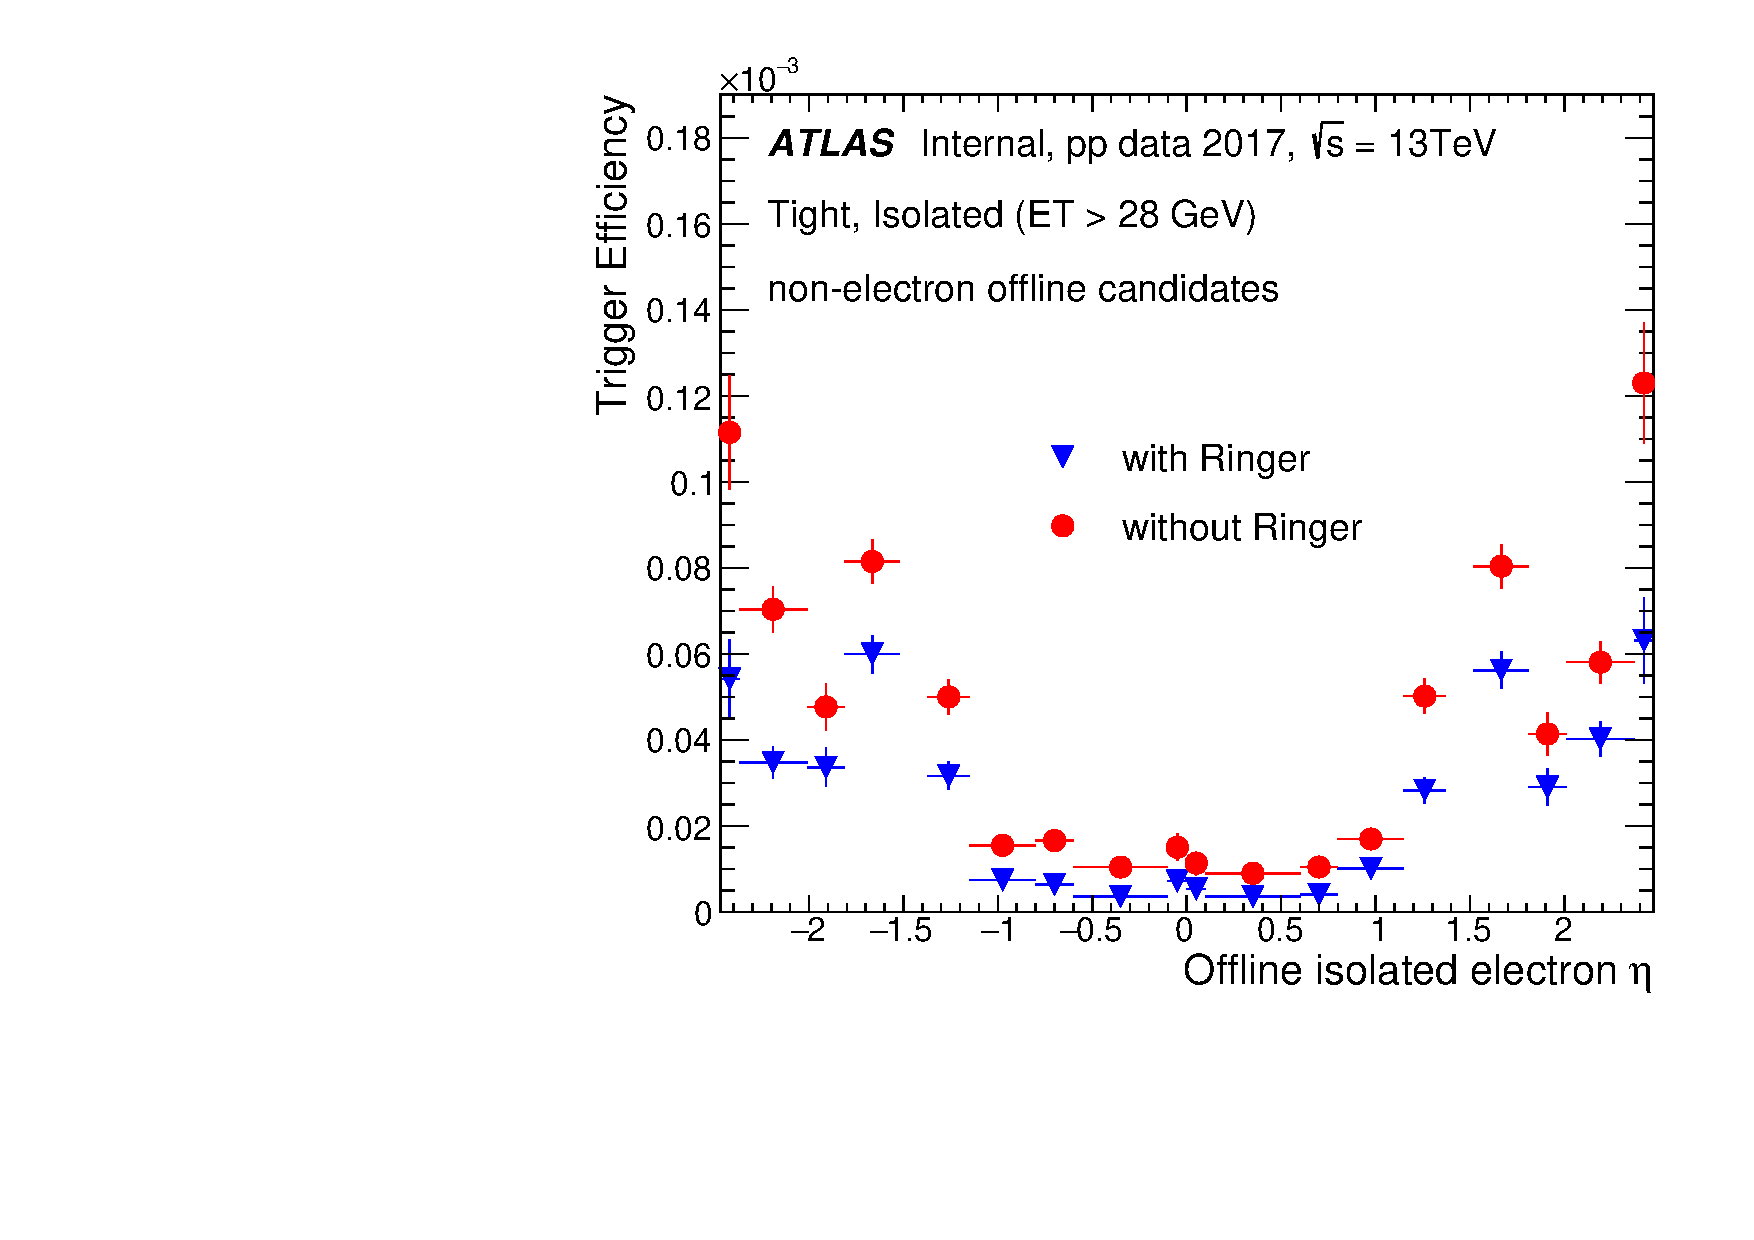
\includegraphics[width=\textwidth]{figures/efficiencies/eff_EGAM7_e28_ringer_and_noringer_2017_after_ts1_HLT_eta.pdf}
  \caption{}
  \end{subfigure}\\
  
  \caption{Efficiency of selecting background at the FastCalo (left) and at the final HLT decision (right) steps as a function of \ET (top) and $\eta$ (bottom) with a single-isolated-electron trigger requiring $\et > \SI{28}{\GeV}$ and \enquote{tight} selection, with and without the \rnn{} algorithm, employing 2017 collision data collected after the \rnn algorithm deployment.}
  \label{fig:2017_fake_triggers_after_ts1}
\end{figure}

For the 2018 data-taking period, the \rnn{} was retrained using collision data, thereby improving electron identification performance. The signal efficiency of the lowest-transverse-energy-threshold unprescaled trigger increased by approximately 1\%, primarily due to several minor enhancements in the full electron selection applied both online and offline. In parallel, a modest reduction in fake-electron acceptance was observed at the \fastcalo{} stage for certain unprescaled triggers relative to the 2017 post-TS1 configuration. Specifically, the lowest-\ET-threshold triggers ($\ET > 17,26,28$) achieved a reduction factor of 1.19, while the highest-\ET-threshold trigger ($\ET > 60$) reached a more significant reduction factor of 1.69.

%For the 2018 operation, the \rnn{} was retrained using collision data. 
%It was also the case for the final HLT
%selection\footnote{One exception was the \medium{} selection, where the HLT likelihood selection operated in 2018 with the same 2017 tune.}. 

%The signal efficiency of the lowest-transverse-energy-threshold unprescaled trigger increased by about 1\%, mainly from several minor improvements of the full electron selection both online and offline.

%As well as maintaining high electron efficiency, some unprescaled triggers were observed to achieve a small reduction in fake-electron acceptance at the  \fastcalo{} step compared to the 2017 operation after TS1. For the lowest-\ET-threshold trigger ($\ET> 17,26,28$), the fake-electron acceptance was reduced by a factor of 1.19, while for the highest-\ET-threshold trigger ($\ET > 60$), a reduction factor of 1.69 was achieved.

\begin{comment}
\subsection{2017 operation}\label{ssec:2017_ringer_operation}

%A single-electron HLT\_e28\_lhtight\_nod0\_(noringer)\_ivarloose triggers, both with \rnn{} and with cut-based (noringer) algorithms, was employed for monitoring purposes after the first technical stop (TS1).
%This trigger requires an electron candidate with $\ET > 28$~GeV satisfying the \enquote{tight} selection (lhtight\_nod0) with \enquote{loose} isolation criteria (ivarloose)~\cite{TRIG-2018-05}. 
%Signal efficiencies for cut-based and \rnn{} triggers for \tnp{} electron candidates from data taken in 2017, compared in Figure~\ref{fig:2017_e28_after_ts1}, show no significant differences of the order of ew per mille.  between the two algorithms.
%Although a slightly more prominent efficiency loss is observed at large \avgmu{} in Figure~\ref{fig:e28_comp_mu} for the \rnn{} trigger, the electron efficiency was indeed kept nearly the same as a goal of the training of the \rnn algorithm, a strategy validated by this result.
%This loss occurs after the linear threshold correction limit of $\avgmu=40$ was employed during 2017.

A single-electron HLT\_e28\_lhtight\_nod0\_(noringer)\_ivarloose trigger, using both \rnn{} and cut-based (noringer) algorithms, was employed for monitoring purposes following the first technical stop (TS1). This trigger requires an electron candidate with $\ET > 28$~GeV that satisfies the \enquote{tight} selection (lhtight\_nod0) and \enquote{loose} isolation criteria (ivarloose)~\cite{TRIG-2018-05}. 

Signal efficiencies for both cut-based and \rnn{} triggers, evaluated for \tnp{} electron candidates from 2017 data, are compared in Figure~\ref{fig:2017_e28_after_ts1}. The results show no significant differences, on the order of a few per mille, between the two algorithms. 

Although a slight efficiency loss is observed at higher \avgmu{} values in Figure~\ref{fig:e28_comp_mu} for the \rnn{} trigger, the overall electron efficiency was maintained nearly constant, consistent with the objective of the \rnn{} algorithm’s training. This strategy is further validated by the results. 

The observed efficiency loss occurs after the application of the linear threshold correction at $\avgmu=40$ during 2017.


Other important triggers were assessed by comparing the trigger efficiencies in 2017 collision data collected before and after switching to the \rnn{} algorithms, as shown in Figure~\ref{fig:2017_electron_triggers}. 
The HLT\_e17\_lhvloose\_nod0\_L1EM15VHI trigger requires an electron candidate with $\ET > 17$~GeV, seeded by the first-level trigger L1\_EM15VHI, and satisfying the loosest identification criteria (lhvloose). 
On the other hand, HLT\_e26\_lhtight\_nod0\_ivarloose requires an electron candidate with $\ET>26$~GeV satisfying \enquote{tight} identification (lhtight) with \enquote{loose} isolation (ivarloose), and HLT\_e60\_lhmedium\_nod0 requires an electron candidate with $\ET>60$~GeV satisfying \enquote{medium} identification (lhmedium). 
The electron efficiency was also kept nearly unchanged for these relevant single-electron triggers. 
As mentioned above, the results in Figure~\ref{fig:2017_electron_triggers} are computed for two different data-taking periods: one with, and the other without, the \rnn{} algorithm. 



\begin{figure}[h!tb]
  
  \begin{subfigure}[c]{.49\textwidth}
  \centering
  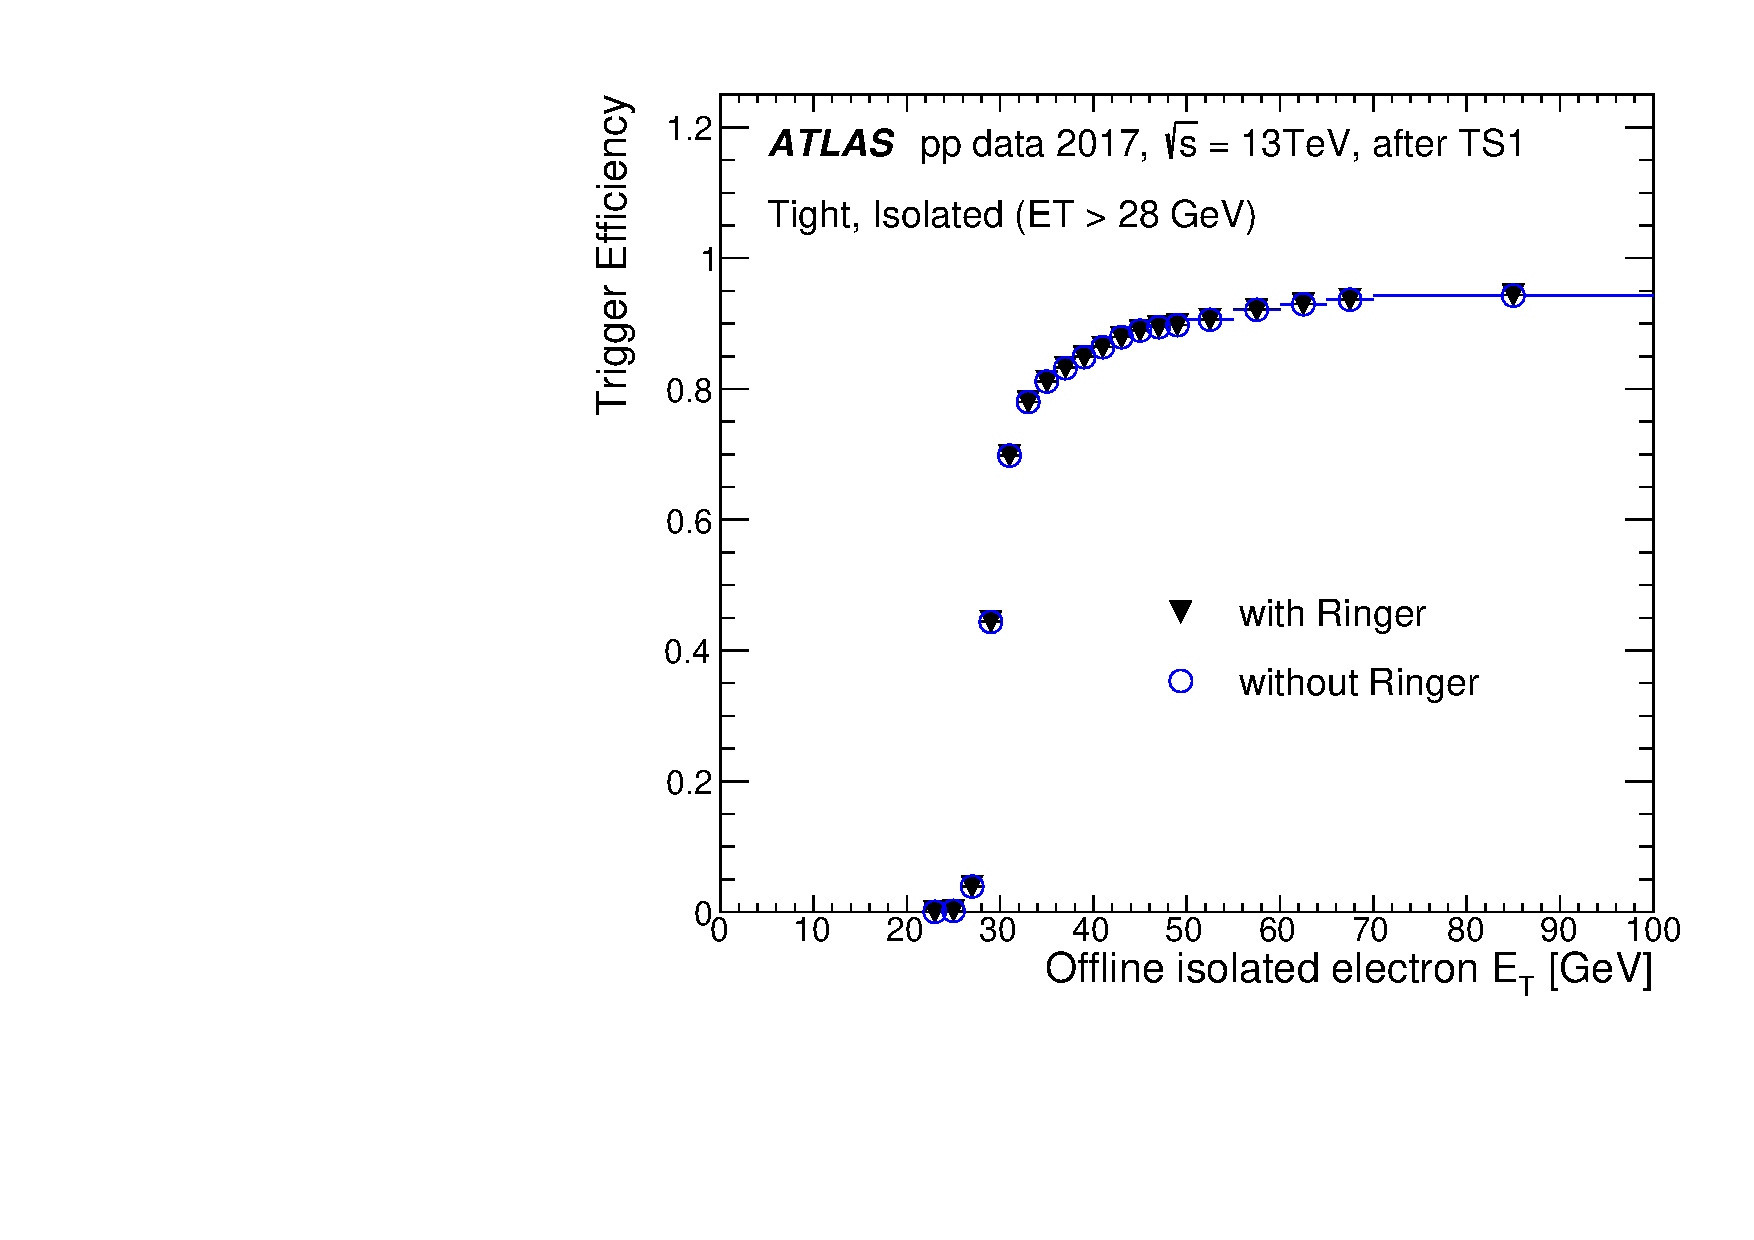
\includegraphics[width=\textwidth]{figures/efficiencies/eff_EGAM1_e28_ringer_and_noringer_2017_after_ts1_HLT_et.pdf}
  \caption{}
  \end{subfigure}
  %
  \begin{subfigure}[c]{.49\textwidth}
  \centering
  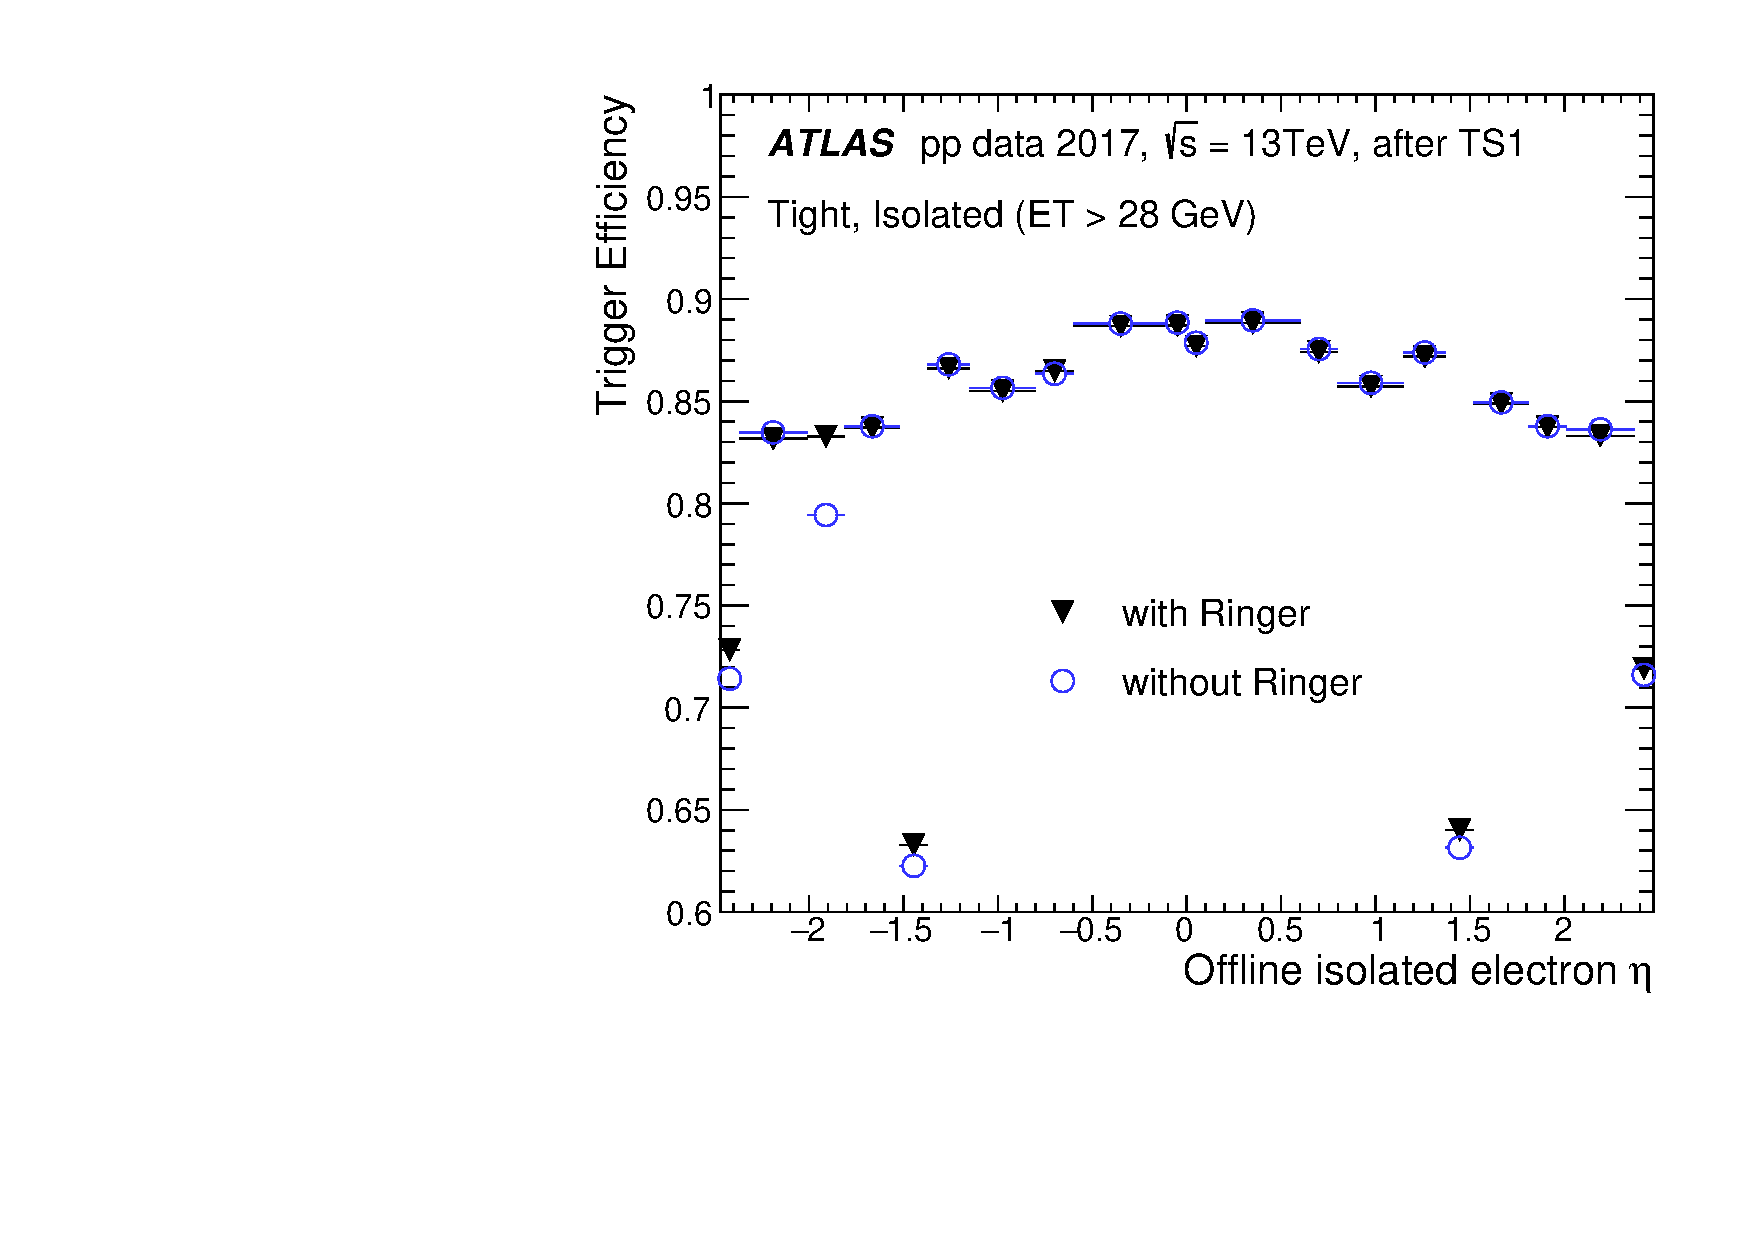
\includegraphics[width=\textwidth]{figures/efficiencies/eff_EGAM1_e28_ringer_and_noringer_2017_after_ts1_HLT_eta.pdf}
  \caption{}
  \end{subfigure}\\
  %
  \centering
  \begin{subfigure}[c]{.49\textwidth}
  \centering
  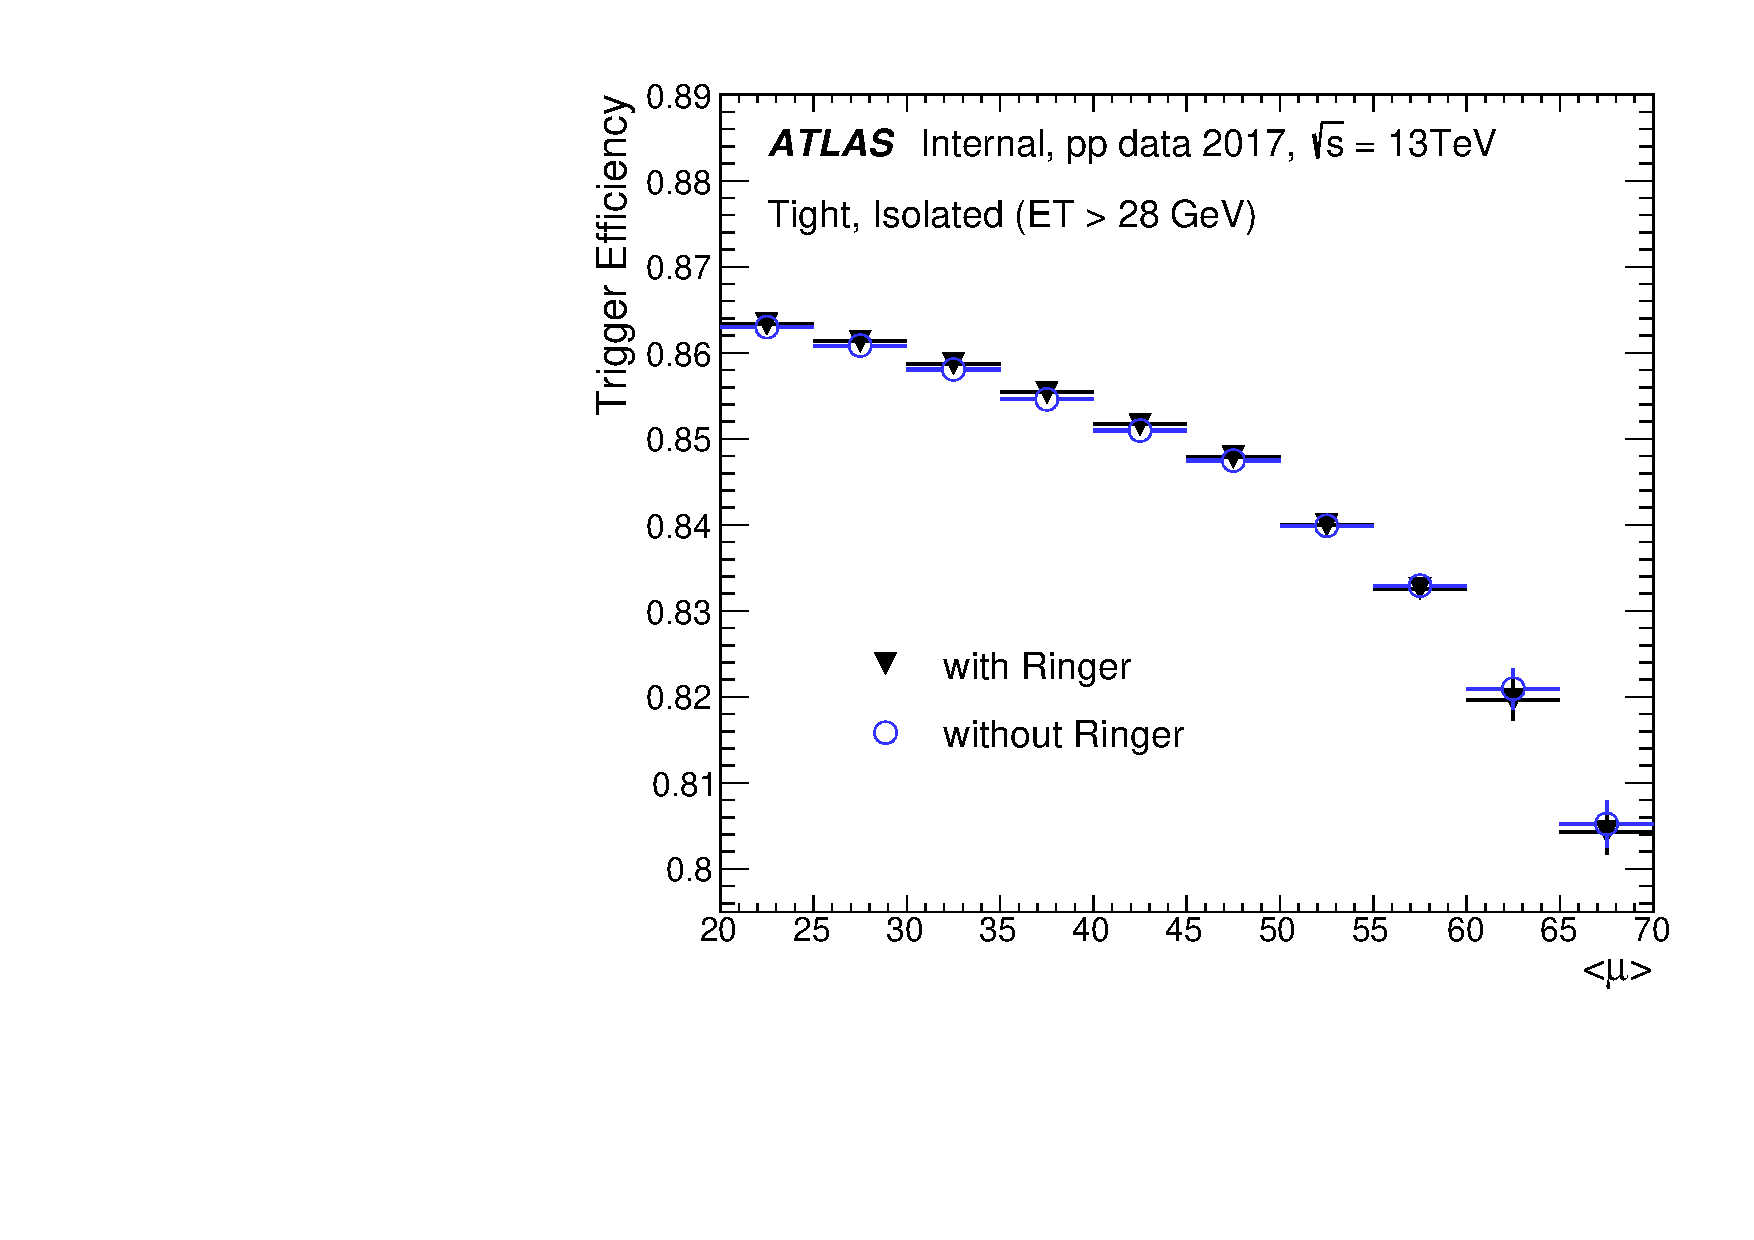
\includegraphics[width=\textwidth]{figures/efficiencies/eff_EGAM1_e28_ringer_and_noringer_2017_after_ts1_HLT_mu.pdf}
  \caption{}%
  \label{fig:e28_comp_mu}
  \end{subfigure}
  
  \caption{
     The efficiency of single-isolated-electron triggers with the \rnn{} algorithm and with the cut-based algorithms as a function of the offline electron (a) \et{}, (b) \eta{}, and (c) \avgmu{} requiring $\et{} > \SI{28}{\GeV}$ after its deployment in July 2027 (TS1). Efficiency is given with respect to offline Tight identification working point. For (b) and (c), only offline candidates with $\et{} > \SI{29}{\GeV}$ are used.
  }
  \label{fig:2017_e28_after_ts1}
\end{figure}




\begin{figure}[h!tb]
  
 \begin{subfigure}[c]{.49\textwidth}
  \centering
  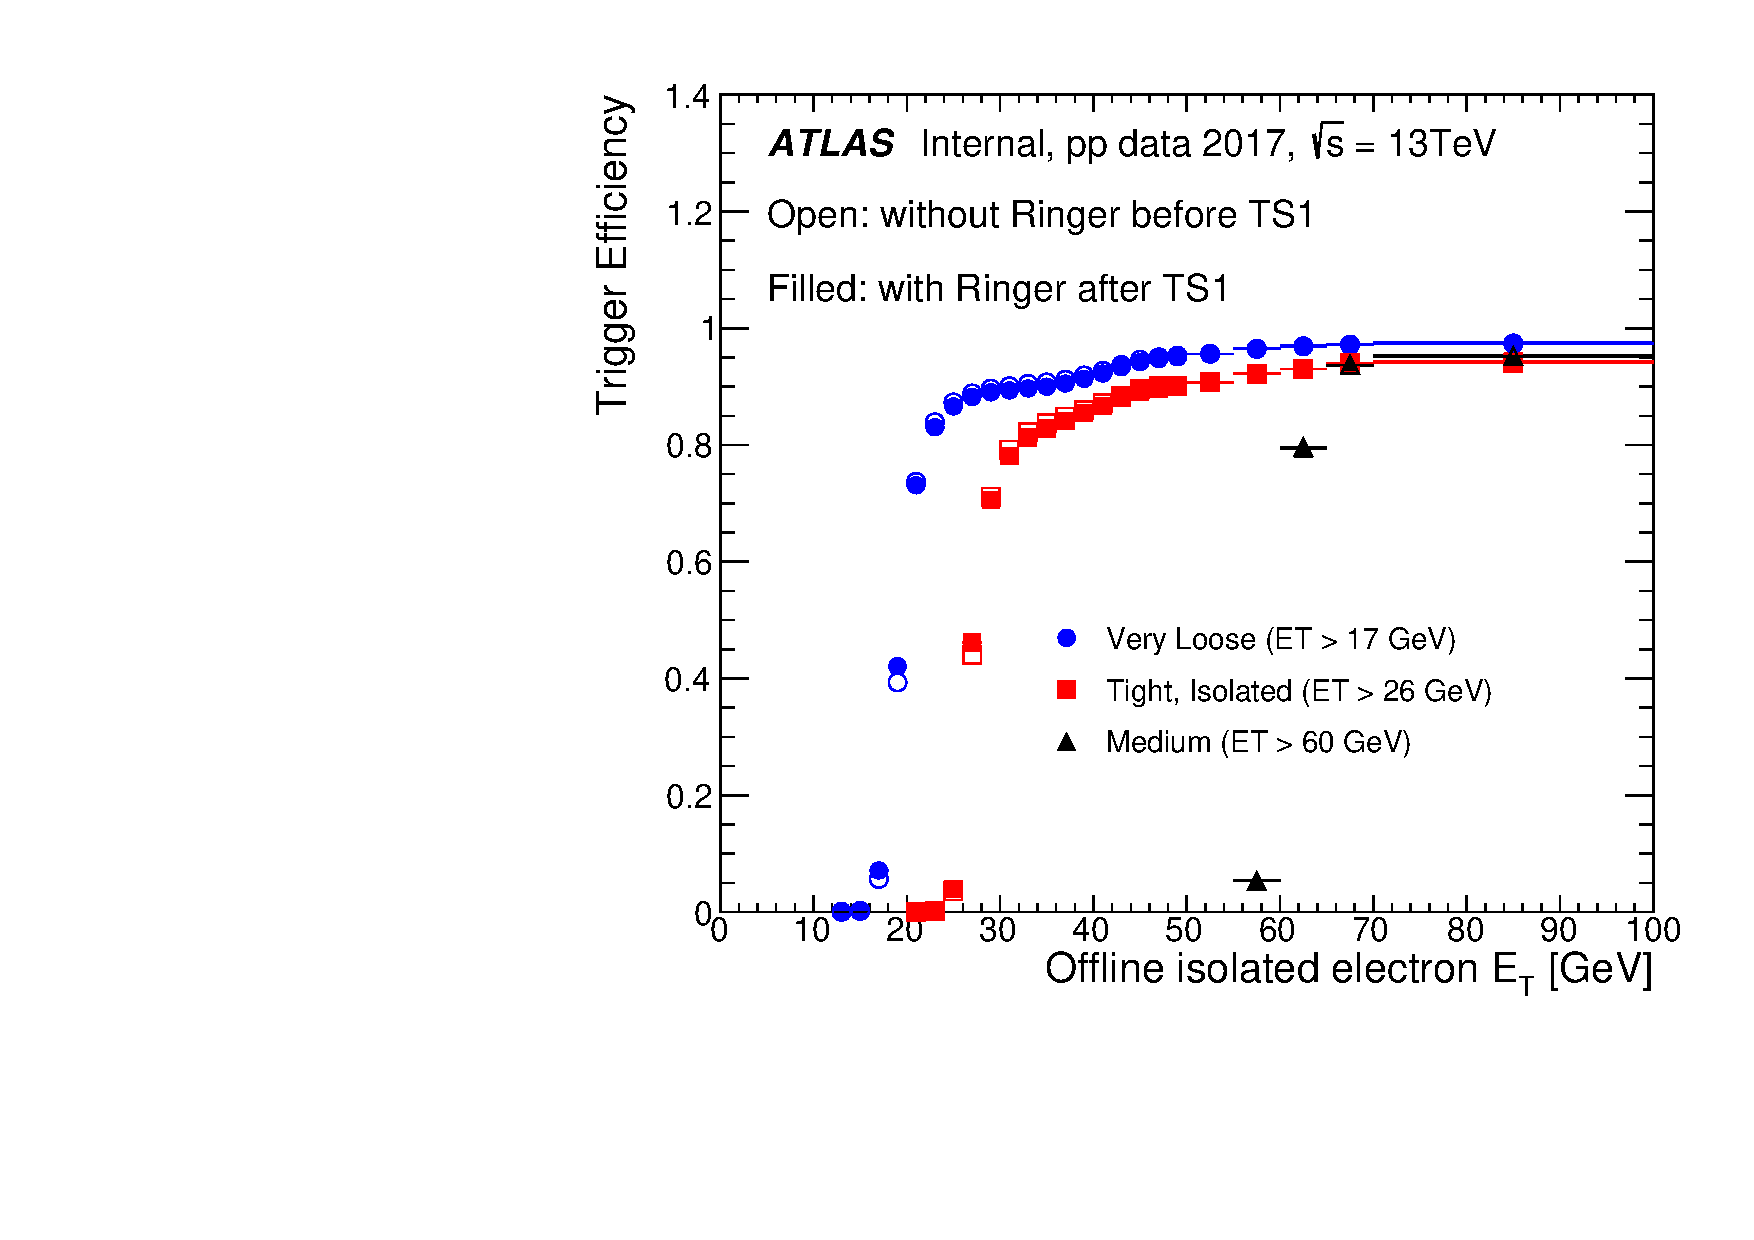
\includegraphics[width=\textwidth]{figures/efficiencies/eff_EGAM1_e17_e26_e60_2017_before_and_after_ts1_et.pdf}
  \caption{}%
  \end{subfigure}
  %
  \begin{subfigure}[c]{.49\textwidth}
  \centering
  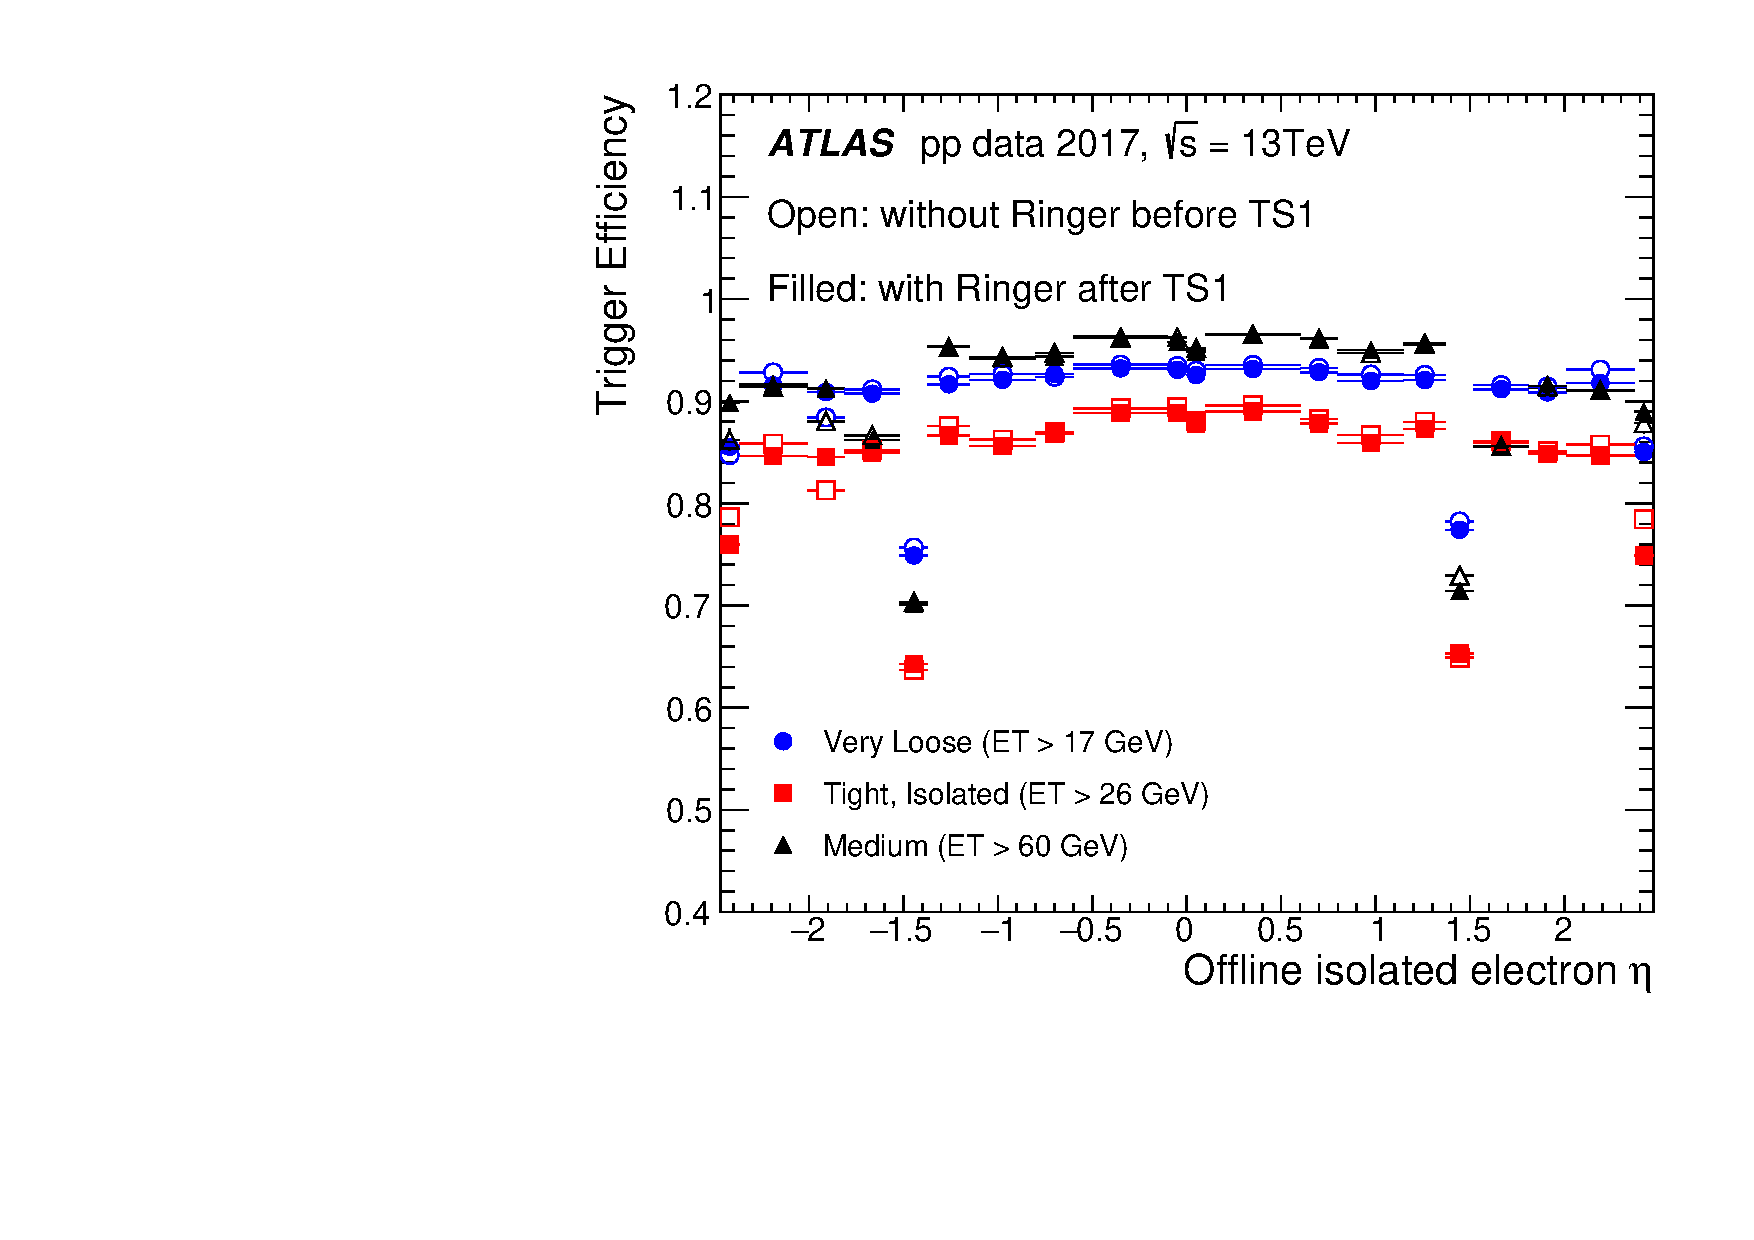
\includegraphics[width=\textwidth]{figures/efficiencies/eff_EGAM1_e17_e26_e60_2017_before_and_after_ts1_eta.pdf}
  \caption{}%
  \end{subfigure}
  
  \caption{
  Efficiency of three single-electron triggers as a function of (a) \et and (b) \eta for 2017 collision data. Open (filled) markers show the efficiency measurements in runs before (after) the deployment of the \rnn{}, thus referring to triggers executed without (with) the \rnn{} algorithm.}
  \label{fig:2017_electron_triggers}
\end{figure}




The power of the \rnn{} algorithm is made clear by examining the behaviour of the duplicated trigger for fake electron candidates in collision data. 
The overall fake-electron rate is reduced by a factor of 13.75 at the \fastcalo step. It can be seen on the left side of Figure~\ref{fig:2017_fake_triggers_after_ts1} that the improvement at the \fastcalo step is similar for all
regions in the evaluated variables, which is particularly interesting when
considering the low \et{} and endcap regions. Besides improving early fake-electron rejection, use of the \rnn{} also resulted in a factor of two reduction in the final fake-electron rate from the HLT
(see right side of Figure~\ref{fig:2017_fake_triggers_after_ts1}), mostly coming from the calorimeter's barrel--endcap transition regions.


\begin{figure}[h!tb]
  \begin{subfigure}[c]{0.49\textwidth}
  \centering
  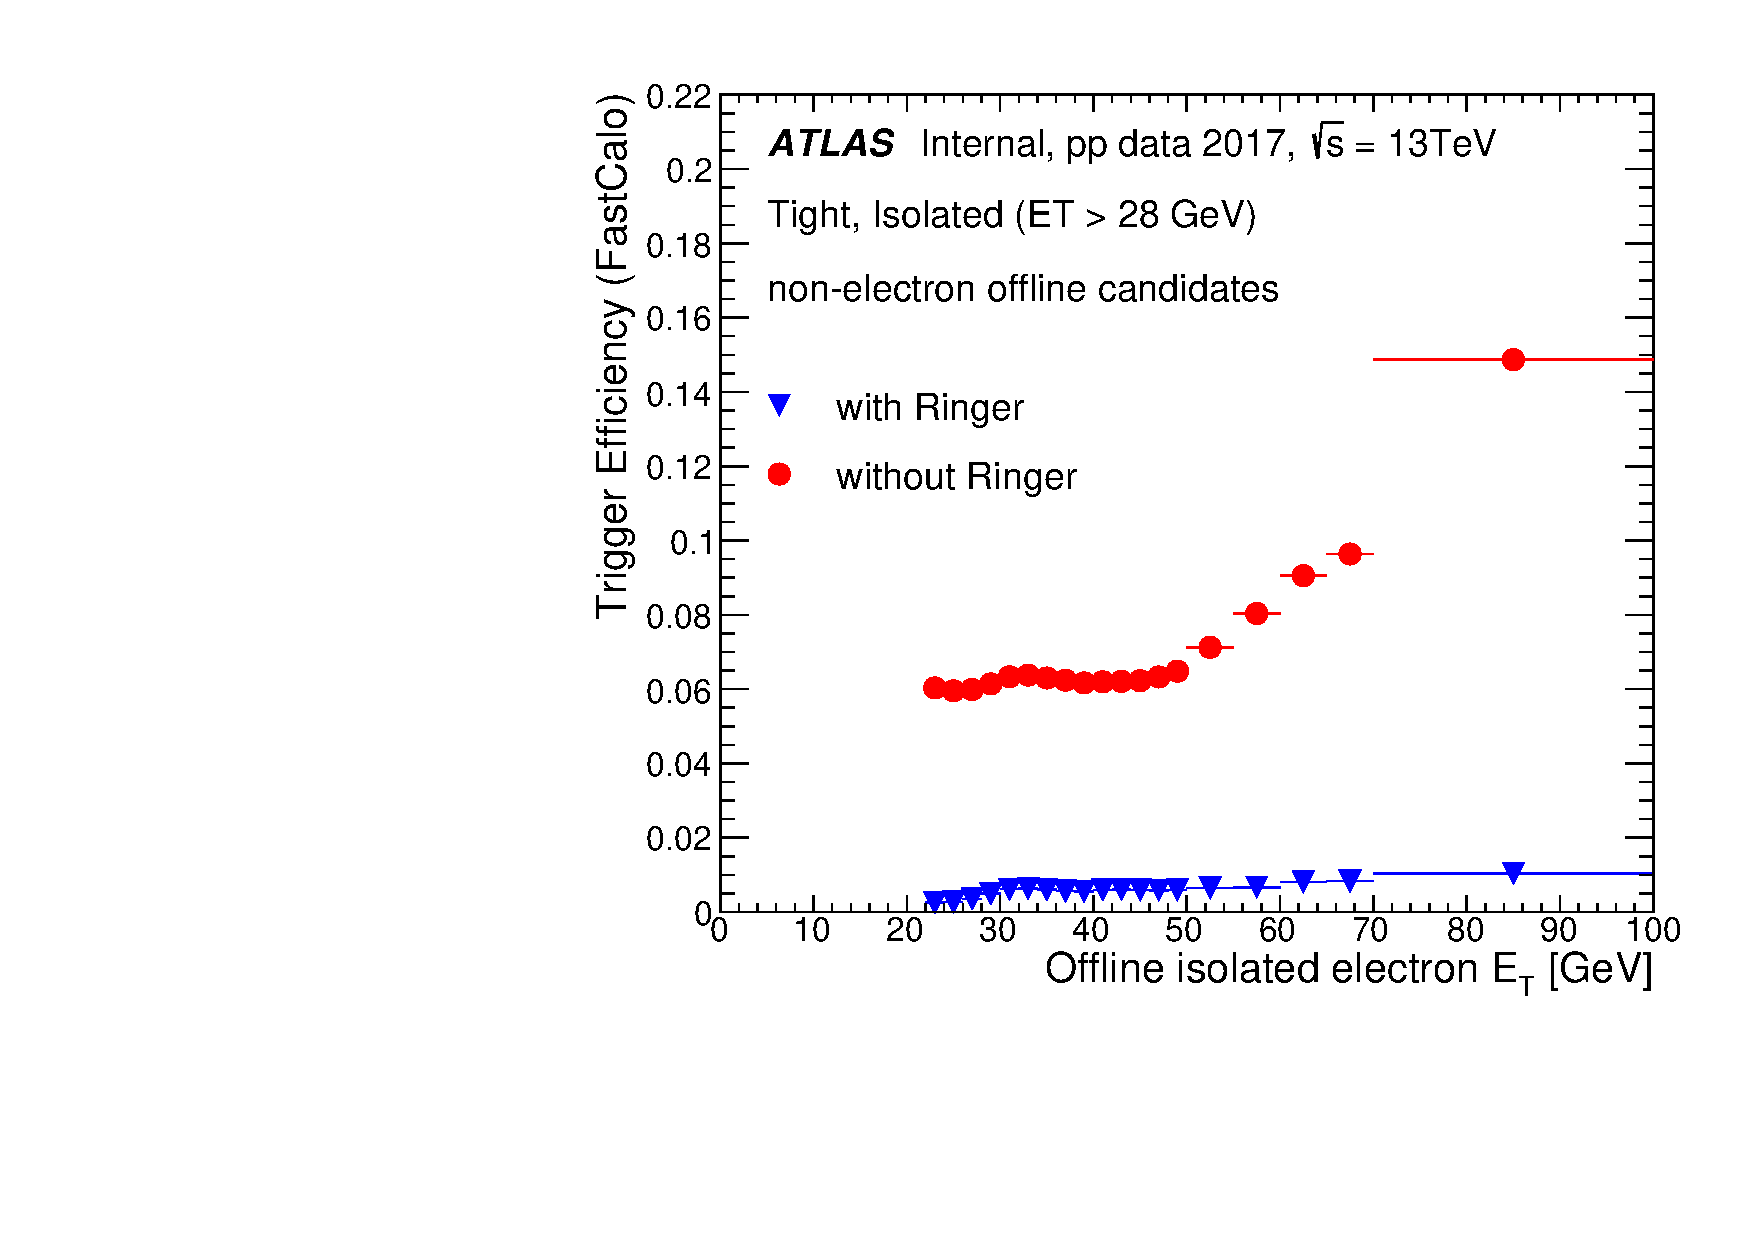
\includegraphics[width=\textwidth]{figures/efficiencies/eff_EGAM7_e28_ringer_and_noringer_2017_after_ts1_L2Calo_et.pdf}
  \caption{}
  \end{subfigure}
  %
  \begin{subfigure}[c]{.49\textwidth}
  \centering
  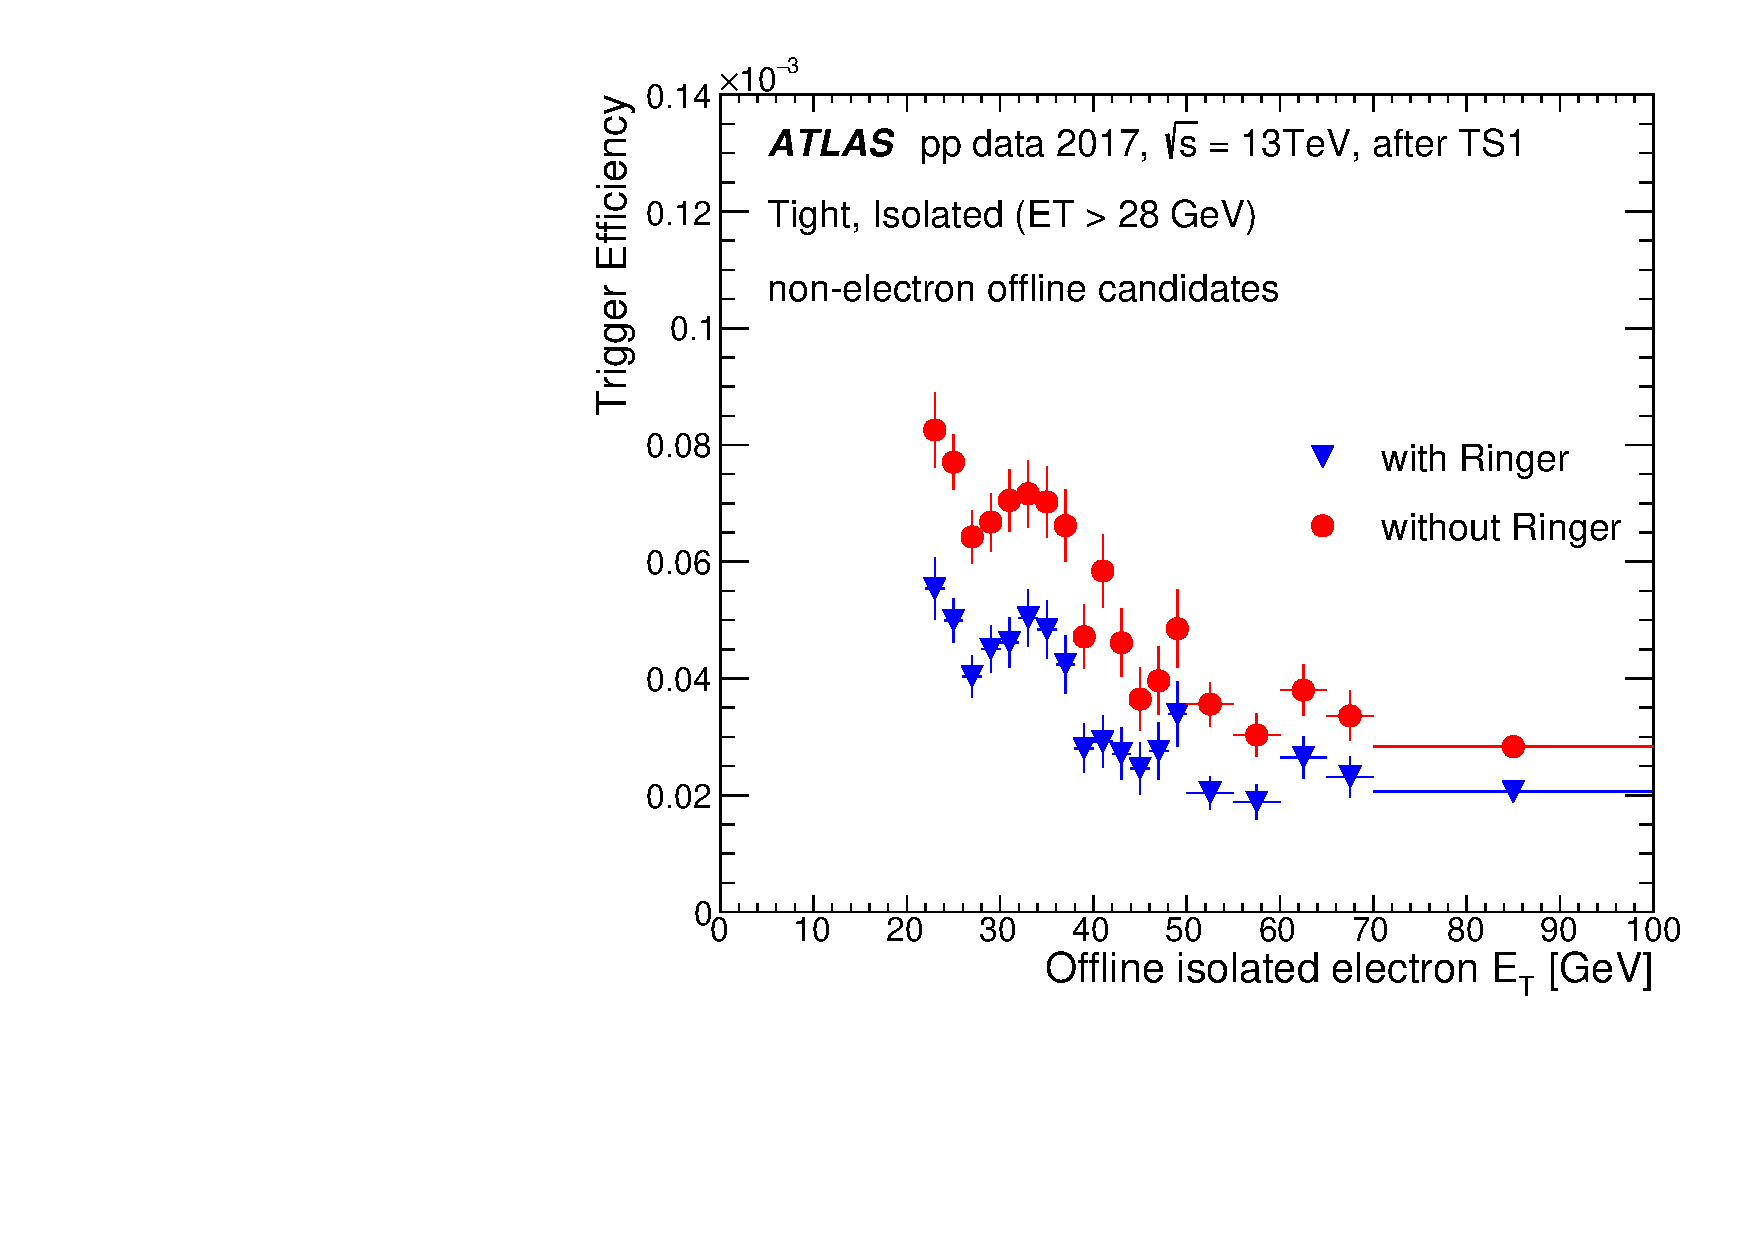
\includegraphics[width=\textwidth]{figures/efficiencies/eff_EGAM7_e28_ringer_and_noringer_2017_after_ts1_HLT_et.pdf}
  \caption{}
  \end{subfigure}\\
  %
  \begin{subfigure}[c]{.49\textwidth}
  \centering
  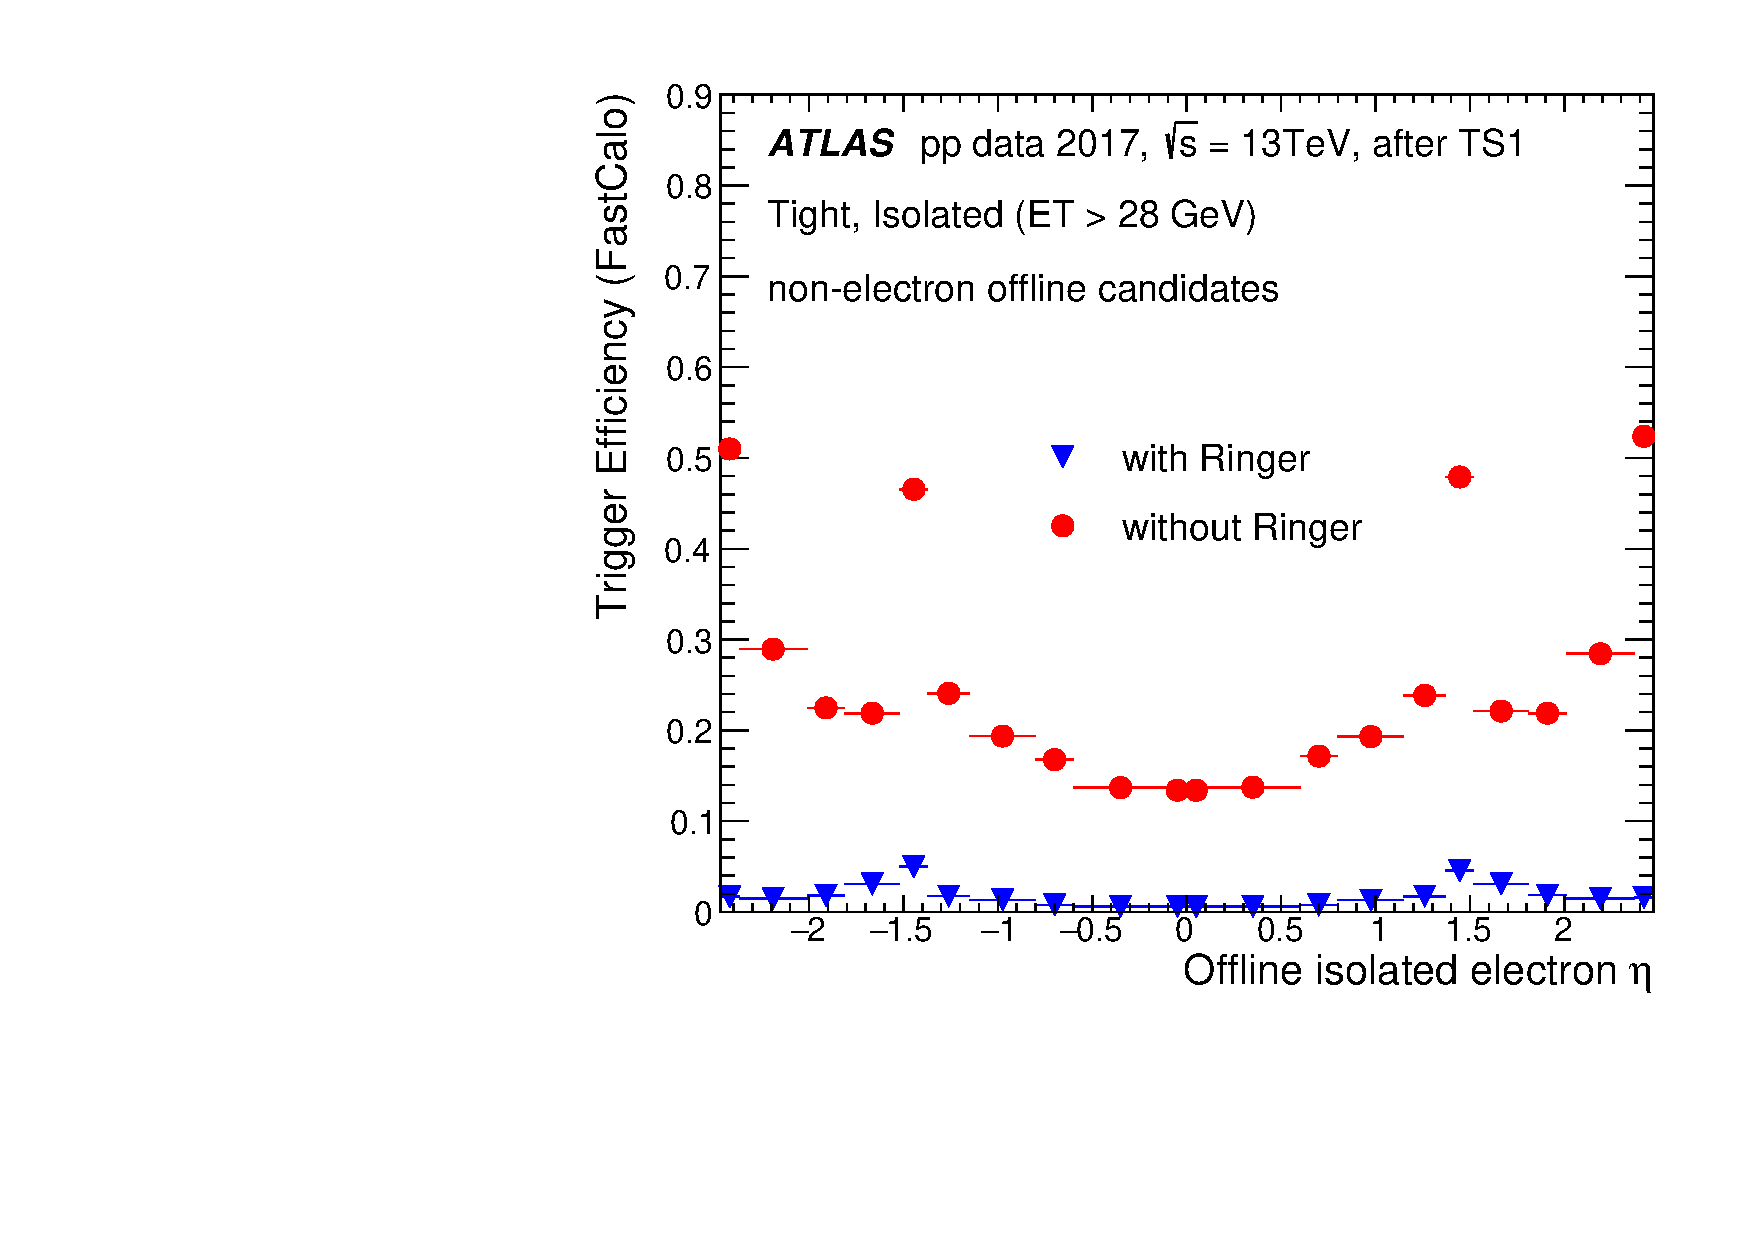
\includegraphics[width=\textwidth]{figures/efficiencies/eff_EGAM7_e28_ringer_and_noringer_2017_after_ts1_L2Calo_eta.pdf}
  \caption{}
  \end{subfigure}
  %
  \begin{subfigure}[c]{.49\textwidth}
  \centering
  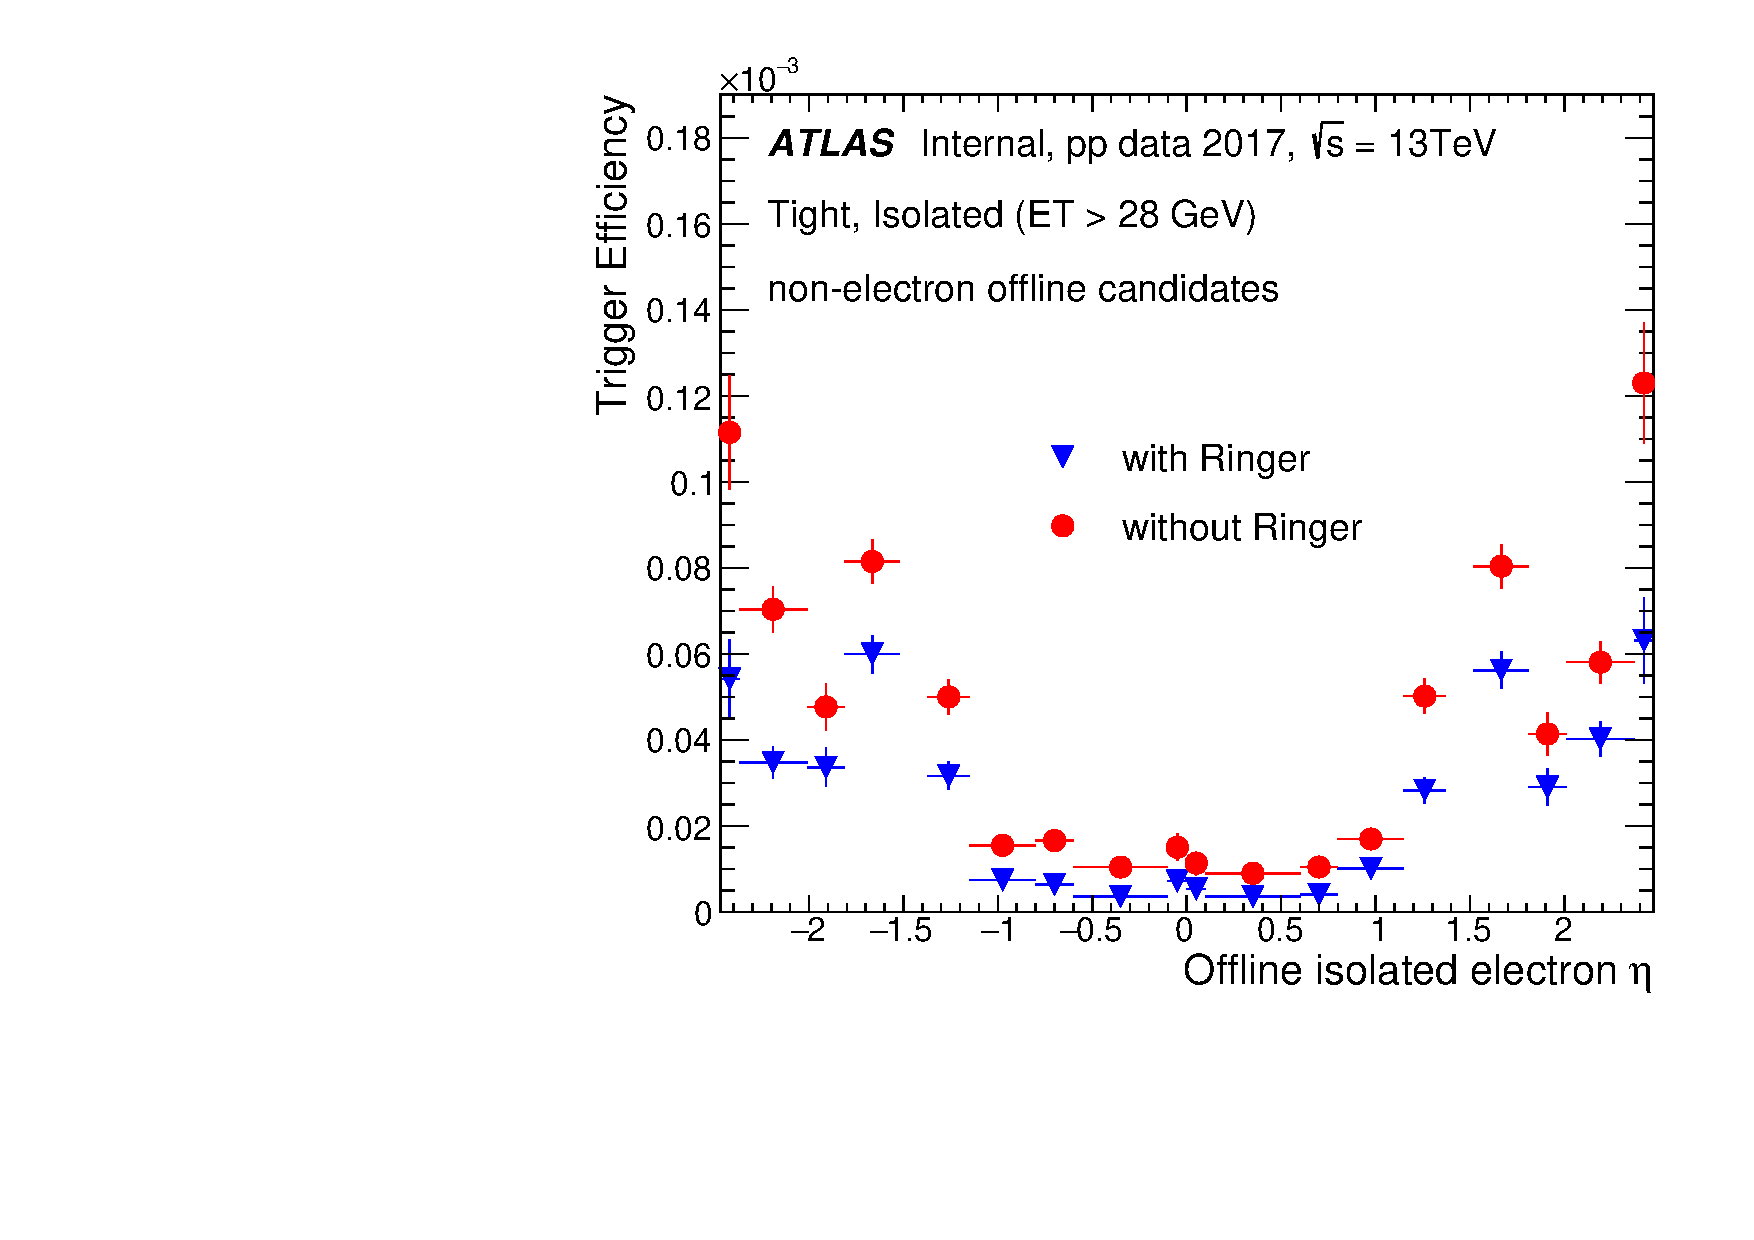
\includegraphics[width=\textwidth]{figures/efficiencies/eff_EGAM7_e28_ringer_and_noringer_2017_after_ts1_HLT_eta.pdf}
  \caption{}
  \end{subfigure}\\
  
  \caption{Efficiency of selecting background at the FastCalo (left) and HLT (right) steps as a function of \ET (top) and $\eta$ (bottom) with a single-isolated-electron trigger requiring $\et > \SI{28}{\GeV}$ and \enquote{tight} selection, with and without the \rnn{} algorithm, employing 2017 collision data collected after the \rnn algorithm deployment.}
  \label{fig:2017_fake_triggers_after_ts1}
\end{figure}

    
\begin{figure}[h!tb]
  \begin{subfigure}[c]{.49\textwidth}
  \centering
  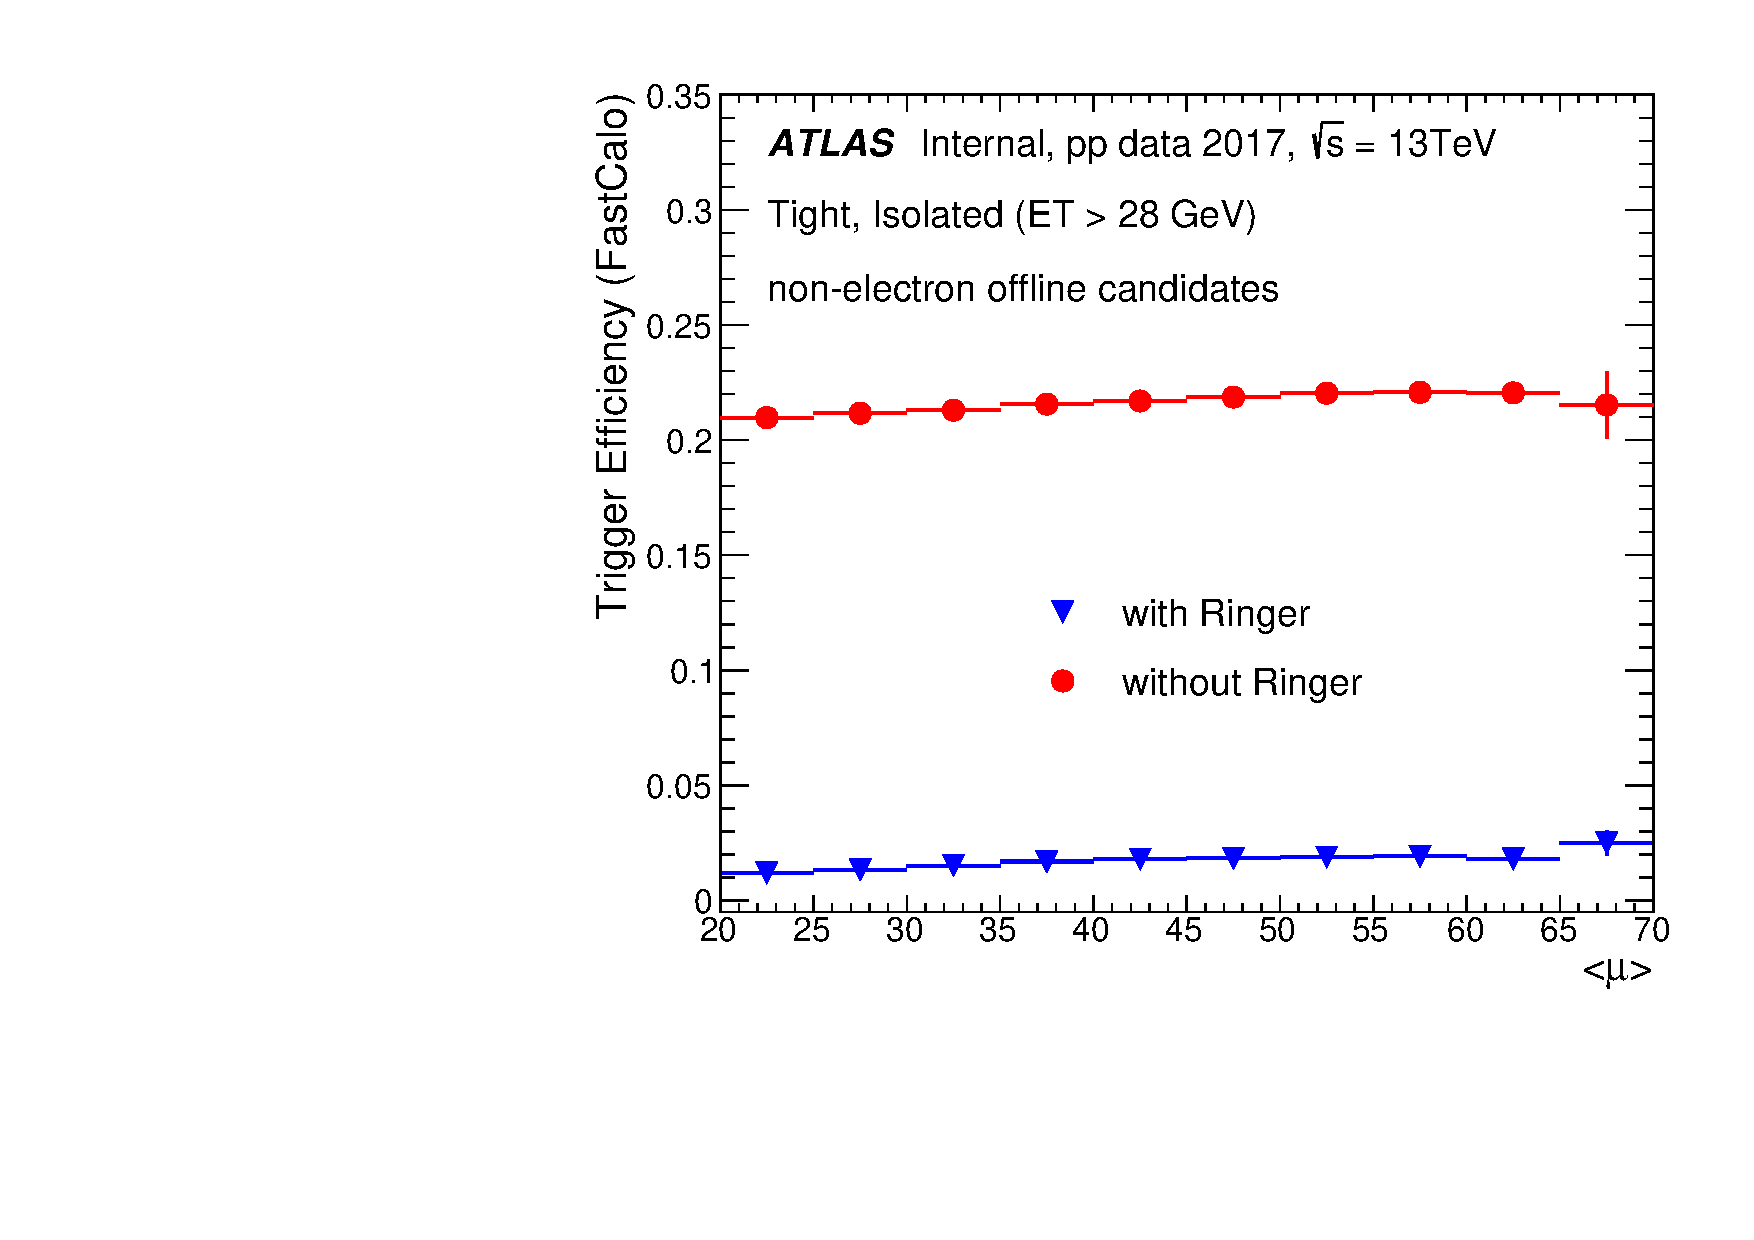
\includegraphics[width=\textwidth]{figures/efficiencies/eff_EGAM7_e28_ringer_and_noringer_2017_after_ts1_L2Calo_mu.pdf}
  \caption{}
  \end{subfigure}
  %
  \begin{subfigure}[c]{.49\textwidth}
  \centering
  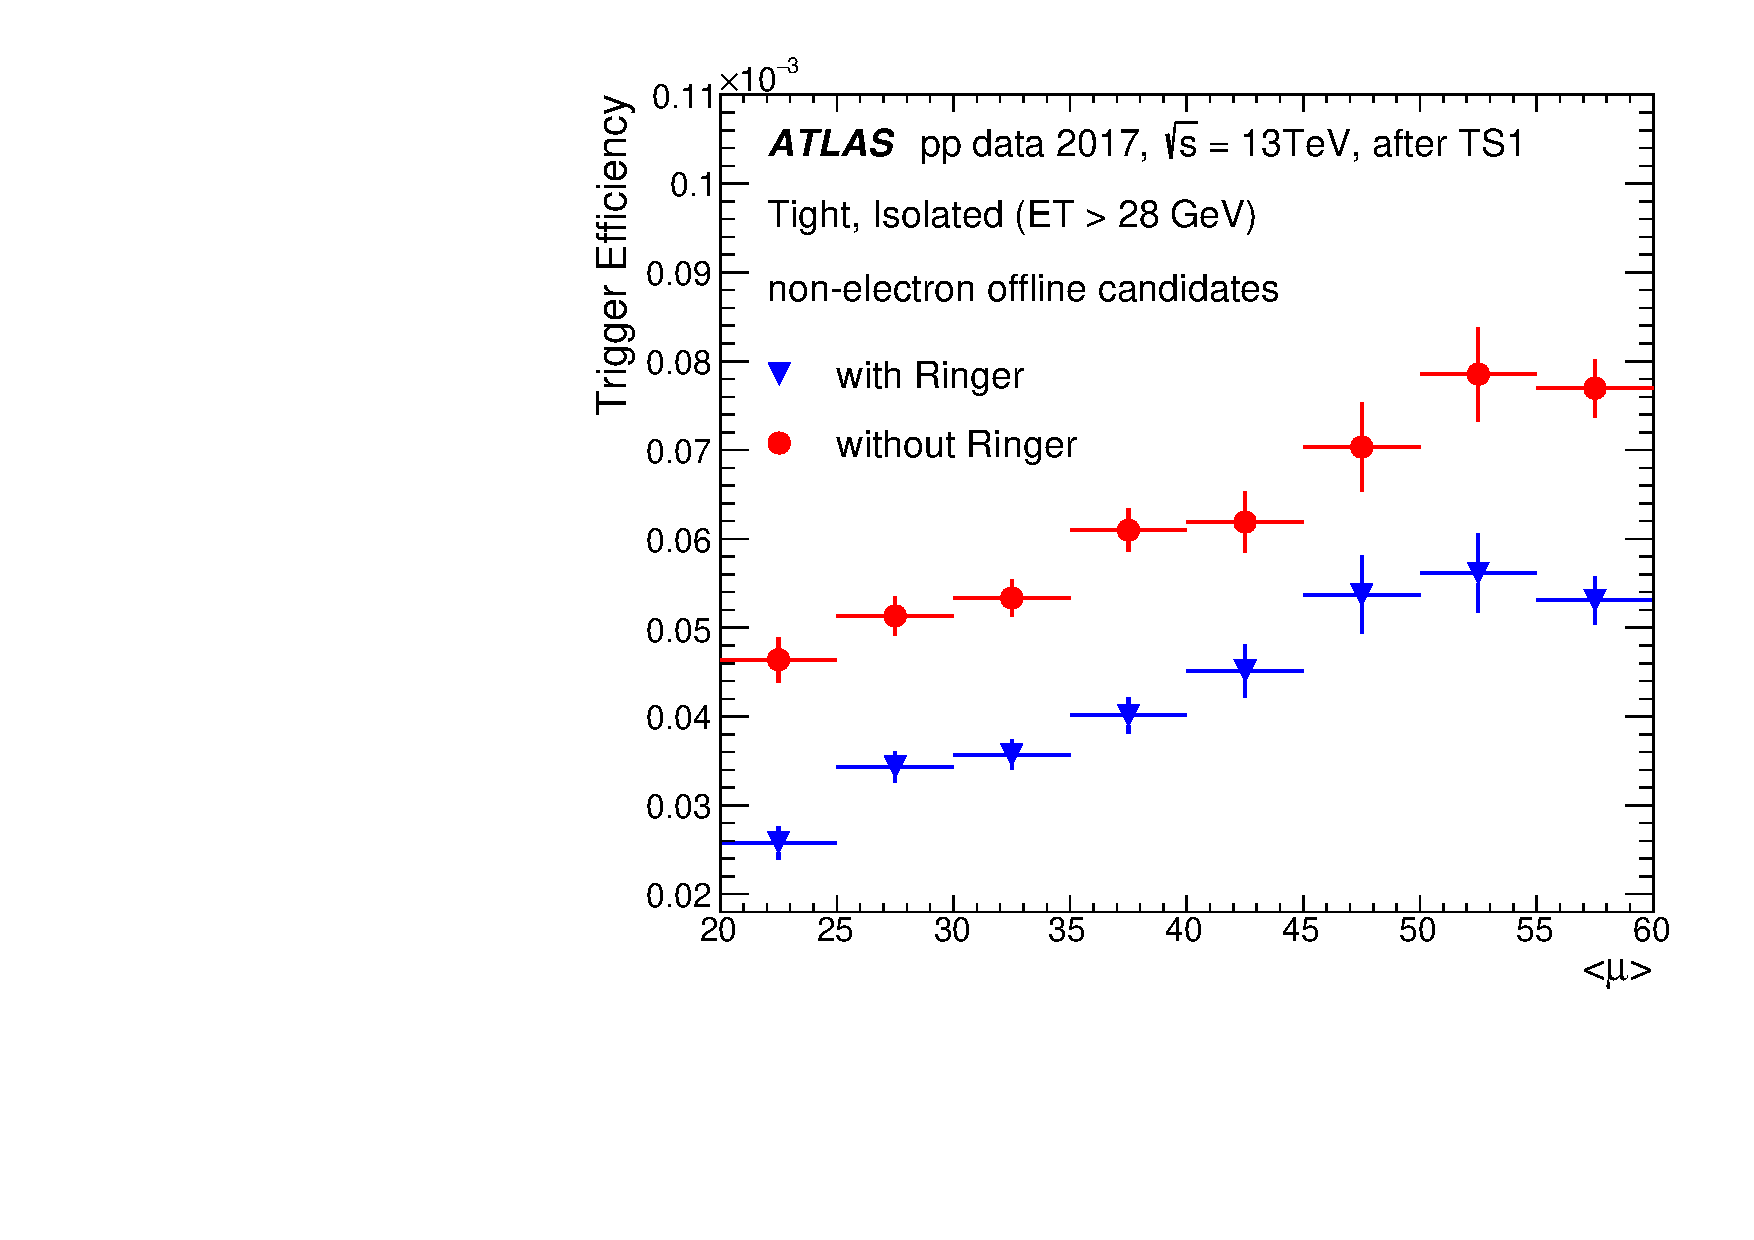
\includegraphics[width=\textwidth]{figures/efficiencies/eff_EGAM7_e28_ringer_and_noringer_2017_after_ts1_HLT_mu.pdf}
  \caption{}
  \end{subfigure}

  \caption{ The single electron isolated trigger requiring $\et > \SI{28}{\GeV}$ and \tight selection with and without the \rnn{} algorithm employing 2017 collision data collected after the \rnn algorithm deployment. Left: \fastcalo fake electron efficiency as a function of \avgmu (a). Right: HLT fake electron efficiency as a function of \avgmu (b).}%
  \label{fig:2017_fake_triggers}
\end{figure}



\subsection{2018 operation}\label{ssec:2018_ringer_operation}

For 2018 operation, the \rnn{} was retrained using collision data. 
%It was also the case for the final HLT
%selection\footnote{One exception was the \medium{} selection, where the HLT likelihood selection operated in 2018 with the same 2017 tune.}. 

The signal efficiency of the lowest-transverse-energy-threshold unprescaled trigger increased by about 1\% mainly from several minor improvements of the full electron selection both online and offline.

As well as maintaining high electron efficiency, some unprescaled triggers were observed to achieve a small reduction in fake-electron acceptance at the  \fastcalo{} step in comparison with 2017 operation after TS1. For the lowest-\ET-threshold trigger (HLT\_e17,26,28 in name), the fake-electron acceptance was reduced by a factor of 1.19, while for the highest-\ET-threshold trigger (HLT\_e60 in name), a reduction factor of 1.69 was achieved.
\end{comment}

\subsection{Impact on CPU demands} \label{ssec:cpu_reduction}


The overhead required to compute the NN decision was evaluated by running the single-isolated-electron trigger requiring $\ET > 17$ GeV trigger with the \rnn algorithm or cut-based approach, in two individual non-concurrent executions using the same dedicated computer system\footnote{This performance study was performed using a Xeon Phi 7120 (1.7 GHz, 32 threads) node with a memory of 256 GB@1333 running a SL6 Operating System.} on the 2017 Enhanced bias~\cite{ATL-DAQ-PUB-2016-002} (EB) data. Hence, the measurements are performed under representative pile-up and topological conditions, with the reconstruction algorithm applied to multiple RoIs in the same bunch-crossing event.

To avoid a complete re-implementation of the \fastcalo trigger step, electron triggers using \rnn{} information make their decision after cut-based features are reconstructed. In this case, the cut-based decision is not computed. This strategy also allows us to continue using cut-based chains for monitoring purposes. As a result, the \rnn{} electron triggers always require additional \fastcalo processing time. Figures~\ref{fig:fastcalo_fex_time} and~\ref{fig:fastcalo_hypo_time} show comparisons of the total processing time per call for the feature extraction and hypothesis-testing algorithms in the \fastcalo step, respectively (see the related \fastcalo blocks in Figure~\ref{fig:electron_chain}). 


\begin{figure}[h!tb]
	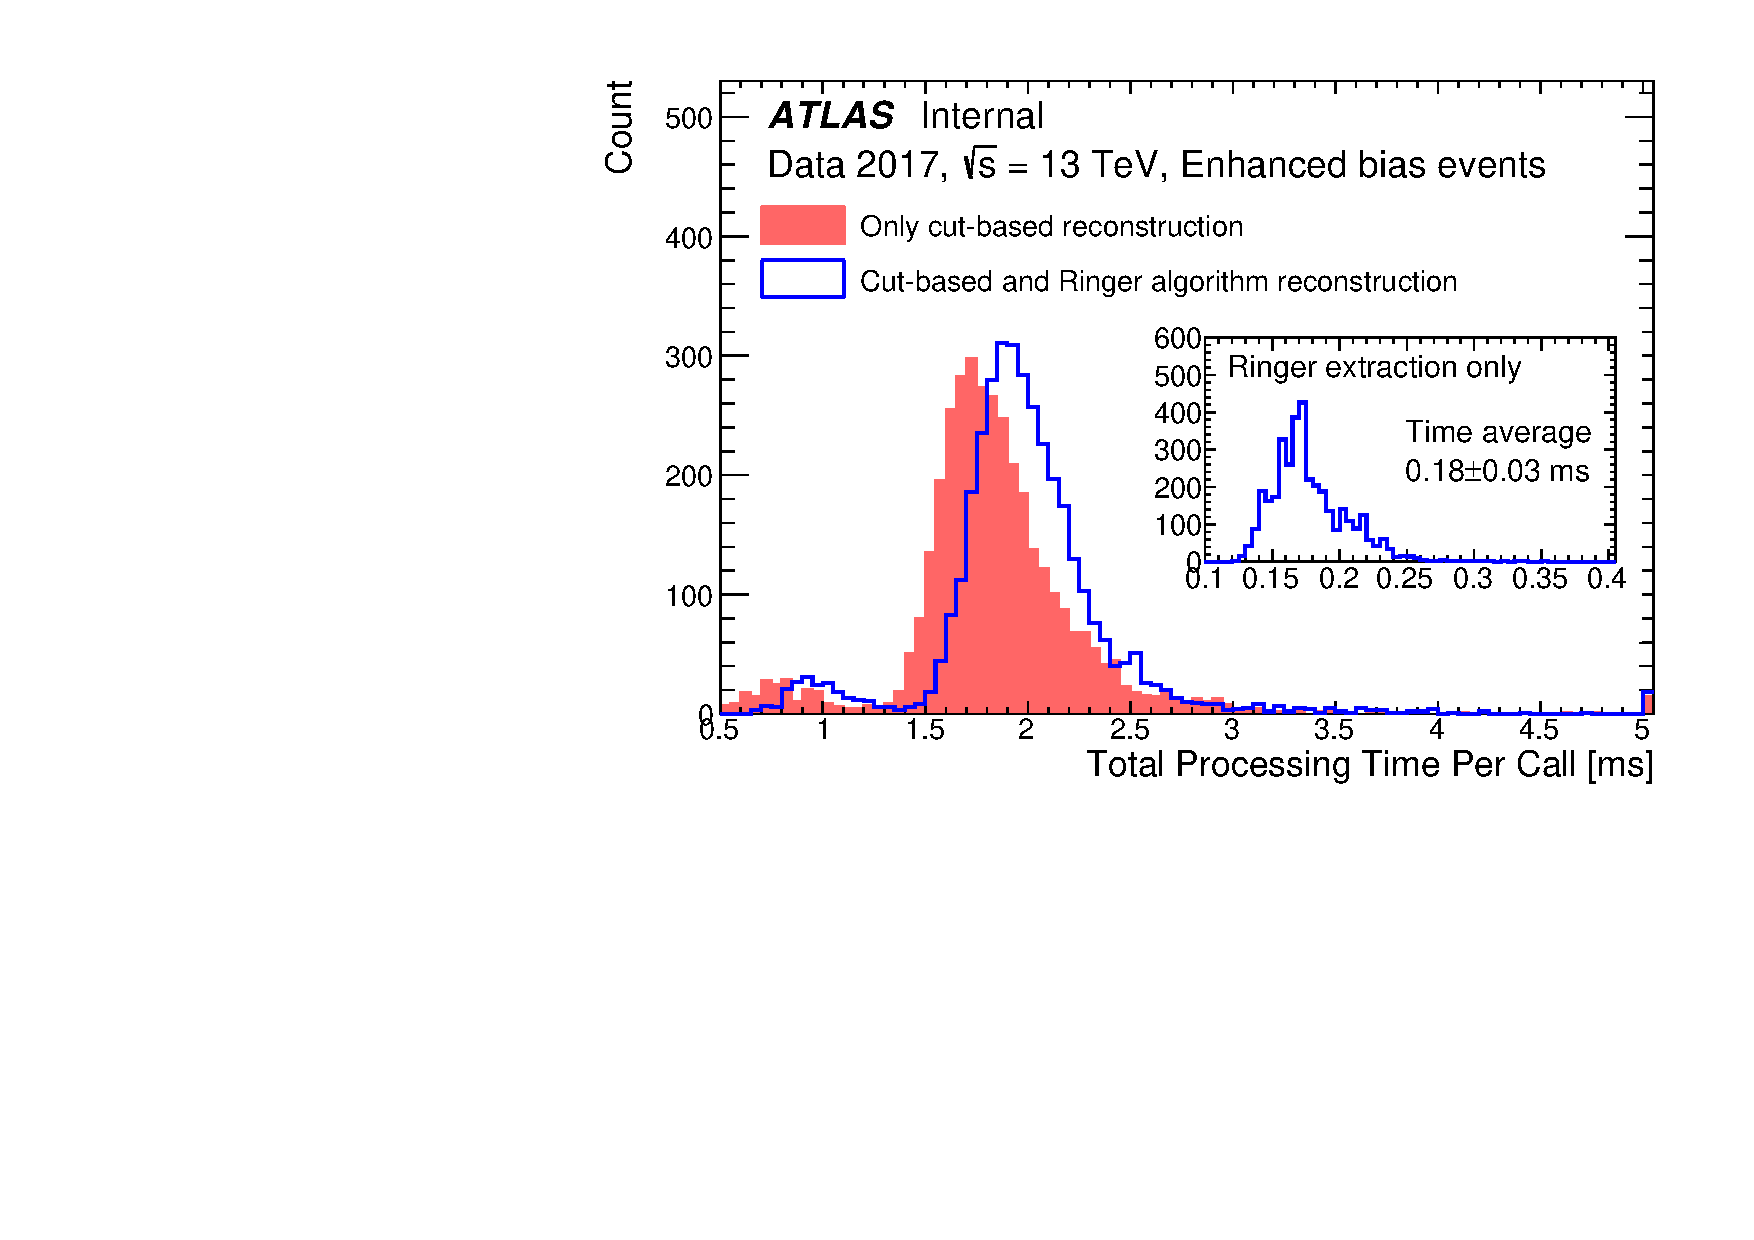
\includegraphics[width=.7\textwidth]{figures/EgammaFex_TotalTime}
	\centering
	\caption{\label{fig:fastcalo_fex_time}
		Total processing time per call for the feature extraction algorithms in the \fastcalo step of an electron trigger requiring $E_T>17$ GeV and Loose identification criteria, with the \rnn (blue) or the cut-based approach (red), on EB events (peak $\avgmu=45$). The inset on the right shows the processing time per call for the ring variable extraction only.  
	}
\end{figure}

\begin{figure}[h!tb]
	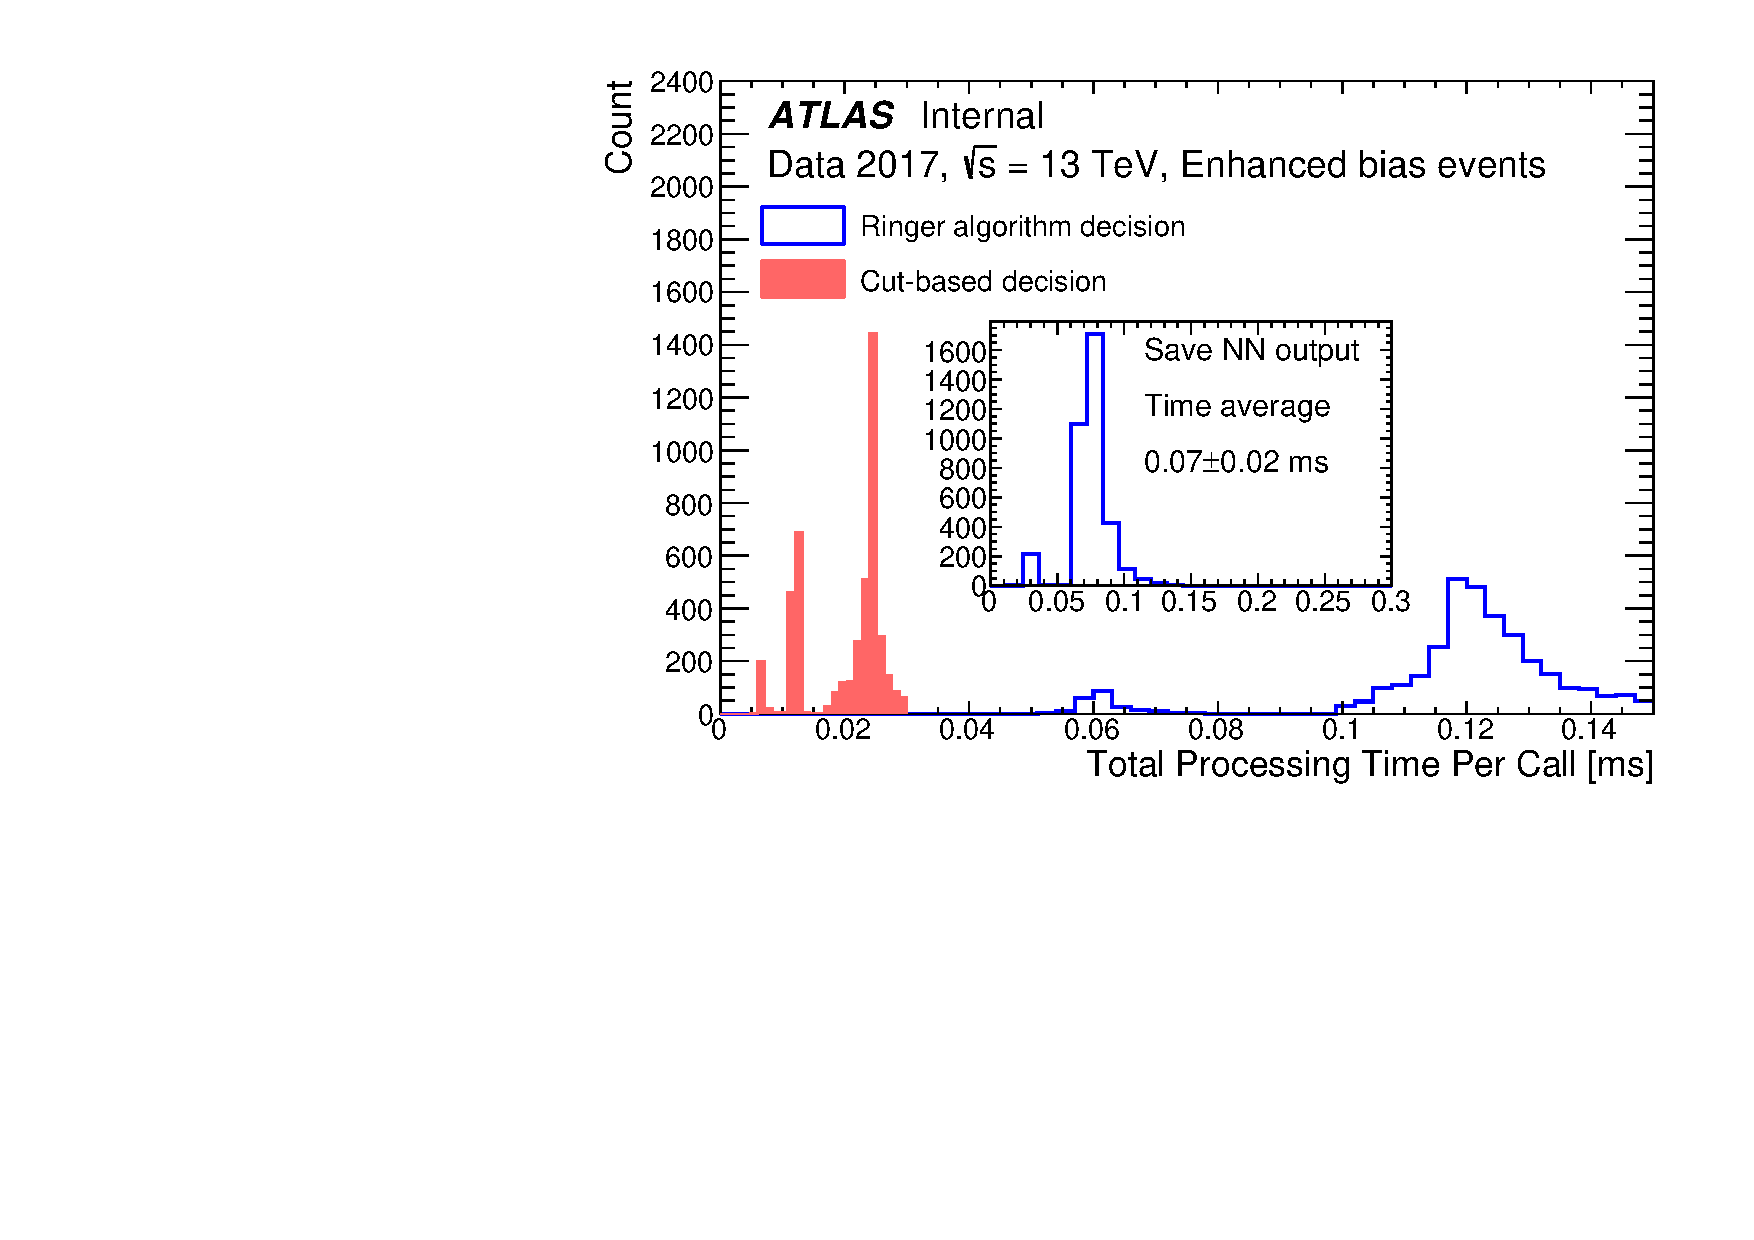
\includegraphics[width=.7\textwidth]{figures/EgammaHypo_TotalTime.pdf}
	\centering
	\caption{\label{fig:fastcalo_hypo_time}
		Total processing time per call for the hypothesis-testing algorithms
		in the \fastcalo step of an electron trigger requiring $E_T>17$ GeV and Loose identification criteria,  with the \rnn (blue) or the cut-based approach (red), on EB events (peak $\langle \mu \rangle = 45$). 
		The center histogram shows the processing time per call to store the entire \rnn{} output in a persistent file format.}
\end{figure}

A multi-modal structure can be observed in the feature-extraction distributions (see Figure~\ref{fig:fastcalo_fex_time}) for both trigger configurations, and it is associated with the algorithm for retrieving EM2 cell energies and building related shower-shape variables. The computation of the ring variables, which is the only difference between the triggers in the \fastcalo feature extraction, requires an additional average processing time of $0.18 \pm 0.03$~ms/event. 


A smaller contribution comes from hypothesis testing (see Figure~\ref{fig:fastcalo_hypo_time}), in which the ring variables are normalized, the discriminating variable's value is computed, and compared with the selection requirement. %, and stored in a persistent file format. 
%Specifically, hypothesis testing for the \rnn{} is considerably more time-demanding (up to \SI{0.14}{\ms/\text{event}}, mostly due to taking   $0.07 \pm 0.02$~ms/event to store the neural-network output) than the cut-based selection (\SI{0.02}{\ms/\text{event}}), but less time-demanding than  feature extraction.
Hypothesis testing for the \rnn{} exhibits significantly higher computational demands than the cut-based selection, with processing times reaching up to \SI{0.14}{\ms/\text{event}}. This overhead is predominantly due to storing the neural network output, which requires $0.07 \pm 0.02$~ms per event. Despite this, the hypothesis testing remains less time-intensive than the feature extraction stage.
Additionally, the time increase is negligible in comparison with the average processing time of a single-electron trigger across the entire HLT ($\approx 500$~ms in \RunTwo).

Taking these values into account, the \rnn{} can require up to \SI{50}{\%} more \fastcalo{} CPU time per event
than the trigger without the \rnn{}.\footnote{The CPU-time increase is expected to depend on the trigger configuration because of the presence of pileup. The reported results are for the single-electron trigger, requiring $\ET > 17$ GeV, with a very loose operation point.} Nonetheless, the \rnn{} provides a more discriminating selection, which reduces the number of CPU-demanding triggers by decreasing the need to process fake electrons in subsequent steps that are more computationally intensive. As shown in previous results (see, for example, Fig~\ref{fig:2017_fake_triggers_after_ts1}), the overall fake-electron rate at the \fastcalo{} step was reduced by a factor of 13.75, preventing these fake events from being processed in the further trigger steps.
%In this measurement, where about 3400 events from the EB stream were considered, the \rnn{} algorithm provided an overall
%\SI{60}{\%} reduction in the CPU demands (from \SI{30.72}{\milli\second} to \SI{10.36}{\milli\second} per event) by rejecting most fake electron candidates during the \fastcalo step. 





